\documentclass[11pt, openany]{book}

\usepackage[top=20mm, bottom= 30mm, left = 30mm, right = 20mm]{geometry}
\usepackage{amsmath, amssymb, graphicx, color, listings, hyperref}
\usepackage{afterpage, fancyhdr, lastpage, setspace}

\usepackage[toc, page]{appendix}
\usepackage{multirow}
\usepackage[table,xcdraw]{xcolor}

\usepackage{tocbibind}
\usepackage{makecell}

\graphicspath{ {./images/} }

\setcounter{secnumdepth}{4}
\setcounter{tocdepth}{4}
\usepackage{rotating}

\renewcommand{\contentsname}{Table of Contents}

\title{RISC-V Based Microcontroller using Arrow DECA Max 10 FPGA Development Board }

\author{Kaung Min Khant}

\hypersetup{
	colorlinks=true,
	linkcolor=black,
	filecolor=black,
	urlcolor=black,
	pdfpagemode=FullScreen,
	citecolor=black,
}

\newcommand{\insertBlockDiagram}[4]{
	\begin{figure}[!h]
		\centering
		\includegraphics[scale=#2]{/block_diagrams/#1}
		\caption{#3}
		\label{#4}
	\end{figure}
}

\newcommand{\insertWaveform}[4]{
	\begin{figure}[!h]
		\centering
		\includegraphics[width=450px]{/waveforms/#1}
		\caption{#3}
		\label{#4}
	\end{figure}
}

\newcommand{\insertStateMachine}[4]{
	\begin{figure}[!h]
		\centering
		\includegraphics[scale=#2]{/state_machine/#1}
		\caption{#3}
		\label{#4}
	\end{figure}
}

\newcommand{\insertFigure}[4]{
	\begin{figure}[!h]
		\centering
		\includegraphics[scale=#2]{#1}
		\caption{#3}
		\label{#4}
	\end{figure}
}


\newcommand{\insertGraphic}[5]{
	\begin{figure}[!h]
		\centering
		\includegraphics[scale=#2, angle=#3]{/graphics/#1}
		\caption{#4}
		\label{#5}
	\end{figure}
}

\newcommand{\insertCode}[4]{
	\begin{figure}[!h]
		\centering
		\includegraphics[scale=#2]{/codes/#1}
		\caption{#3}
		\label{#4}
	\end{figure}
}

\newcommand{\io}[1]{\underline{\textbf{#1}}}
\newcommand{\sig}[1]{\textbf{#1}}

\fancypagestyle{plain}{%
}

\fancypagestyle{title} {
	\fancyhead{}
	\fancyfoot{}
	\fancyfoot[LO, LE]{6556-6555ELEMM \hspace{1cm} Aug. 2023}
	\renewcommand{\headrulewidth}{0pt}
	\renewcommand{\footrulewidth}{1pt}
}

\renewcommand{\arraystretch}{1.3}
\renewcommand{\bibname}{References}

\newcommand\blankpage{%
    \null
    \thispagestyle{empty}%
    \addtocounter{page}{-1}%
    \newpage}

\begin{document}

\makeatletter
\begin{titlepage}
\thispagestyle{title}
\linespread{1}
	\flushleft
	
\includegraphics[scale = 1]{/graphics/liverpool} \\
	Department of Electronics \& Electrical Engineering / Mechatronics Engineering

	\vspace{1.5in}
  
	\huge{\textbf{\@title}}


	\vspace{1.5in}

	\textbf{Dissertation}

	\vspace{1.5in}

	\textbf{\@author}

	\vspace{0.5in}
	{
    \setstretch{0.1}
    \large
		Supervisor: Dr. Thet Htun Khine\\
		2$^{nd}$ Marker:
	}
\end{titlepage}
\makeatother

\newpage
\renewcommand{\thepage}{\roman{page}}
\setcounter{page}{1}
{
\newpage
\vspace*{\fill}
{
	\centering
	\section*{Acknowledgements}
}
\addcontentsline{toc}{section}{Acknowledgement}
\indent This work would not have been possible without the support of Auston University.
I am especially indebted to Dr. Thet Htun Khine, who have been supportive of my research and who worked actively to provide me with the
protected academic time to meet the required goals.
I am grateful to all of those with whom I have had the pleasure to work during this and other related
projects.

\vspace{0.5cm}
Nobody has been more important to me in the pursuit of this project than the members of my family, and friends. I
would like to thank my parents, whose love and guidance are with me in whatever I pursue. They are the
ultimate role models. Importantly, I wish to thank my friends, Ko Htet Linn Aung, Ko Minn Bo Bo, Ko Naing Lin Aung for support when I damaged
my laptop and when I was stuck during research. 
Futhermore, I would like to deliver graditude to my lovely girlfriend, Ma Shunn Le Yee, who provided me with much needed emotinal
support.
\vspace*{\fill}
}

{
\newpage
\vspace*{\fill}
{
	\centering
	\section*{Abstract}
}
\addcontentsline{toc}{section}{Abstract}
Microcontrollers have become a ubiquitous and vital component in a wide range of applications, from embedded systems to Internet of Things (IoT) devices.
With the growing demand for efficient and versatile computing solutions, the RISC-V (Reduced Instruction Set Computing - V) Instruction Set Architecture (ISA) has emerged as
a promising alternative to proprietary and traditional ISAs.


This thesis presents the design and implementation of a RISC-V microcontroller tailored to meet the demands of modern computing systems.
The proposed microcontroller architecture leverages the inherent advantages of RISC-V, including simplicity, modularity, and extensibility,
to deliver enhanced performance and versatility compared to existing solutions.


The research begins with a comprehensive study of the RISC-V ISA, identifying its key features and design principles.
Based on this analysis, a custom microarchitecture is devised to optimize critical components such as instruction decoding, pipeline stages, and data forwarding mechanisms.
The microcontroller is then synthesized and simulated using industry-standard Electronic Design Automation (EDA) tools to assess its performance, and area utilization.


The results of this research illustrate the feasibility and benefits of employing RISC-V as the foundation for designing microcontrollers.
The proposed architecture's ability to achieve improved performance and adaptability to application-specific
needs lays the groundwork for broader adoption of RISC-V in future computing systems.


In conclusion, this thesis contributes to the growing body of knowledge surrounding RISC-V microcontroller design and serves as a stepping stone for
further advancements in the field of open-source and customizable processor architectures. As RISC-V gains momentum in the industry,
the developed microcontroller has the potential to drive innovation and address the ever-evolving demands of the digital era.
\vspace*{\fill}
}


\pagestyle{fancy}
\thispagestyle{fancy}
\fancyhead{}
\fancyhead[LO, RE]{6556-6555ELEMM}
\fancyhead[RO, LE]{RISC-V Based Microcontroller using Arrow Deca Max 10}
\fancyfoot{}
\fancyfoot[LO, LE]{ Kaung Min Khant - PN1046592}
\fancyfoot[RO, RE]{Page\ \thepage\ of \pageref{LastPage} }
\renewcommand{\headrulewidth}{1pt}
\renewcommand{\footrulewidth}{1pt}

\linespread{1.5}

% \maketitle

\newpage

\tableofcontents

\listoffigures

\listoftables
\newpage
\afterpage{\blankpage}
\renewcommand{\thepage}{\arabic{page}}
\setcounter{page}{1}
\chapter{Introduction}
\section{Project Background}

In recent years, the rapid advancement of technology has led to an exponential growth in the number of embedded systems and Internet of Things (IoT) devices. 
These systems demand efficient, low-power, and versatile microcontrollers capable of executing complex tasks while maintaining cost-effectiveness. 
To address these challenges, the development of a RISC-V-based microcontroller presents an attractive and innovative solution.


The Reduced Instruction Set Computing - V (RISC-V) Instruction Set Architecture (ISA) is an open standard, freely available for anyone to use, modify, and implement. 
Its modular and scalable design has gained significant attention within the semiconductor industry and academic community. 
Unlike proprietary ISAs, RISC-V fosters collaboration and fosters a rich ecosystem of open-source hardware and software projects, 
leading to reduced development costs and increased accessibility.


This project aims to design a RISC-V microcontroller that leverages the benefits of the RISC-V ISA, 
tailored to meet the specific requirements of modern computing applications. The motivation behind this work aims to provide the detail designs of several parts of 
the microcontroller, aiming to act a reference and a base for future design and implementation of the microcontroller core using RISC-V ISA.


\section{Aims and Objectives}
This research is proposed for construction of RISC-V Hardware using VHDL and implemented on FPGA.
The objectives of this research are as follow.
\begin{enumerate}
	\item To build a complete microcontroller, yet simple enough to follow, based on RISC-V RV32E ISA using VHDL.
	\item To offer detail documentation of the implementation of the hardware
	\item To offer hardware extension for future developement
	\item To offer assembler for firmware creation
	\item To offer implementation support for hardware designers to build their own hardwares based on the required projects
\end{enumerate}
\section{Expected Outcomes}
The expected outcomes of the research are as follows
\begin{enumerate}
	\item The CPU must work based on the specified ISA, in this case, RICS-V RV32E ISA
	\item The CPU must be tested
	\item The overall micro-controller must have standard peripherals and they must be tested
	\item The documentation of all of the hardware implements must be provided
	\item The research will be published on GitHub Repo

\end{enumerate}

\section{Report Structure}
This report has been broken down into sections.
\begin{enumerate}
  \item Chapter 1: Introduction - Introduction above this work
  \item Chapter 2: Literature Review - A review of current microcontroller works around RISC-V
  \item Chapter 3: Microcontroller CPU Design and Implementation - RISC-V CPU Core Design and Implementations
  \item Chapter 4: Peripheral Designs and Implementation - Design of peripherals for CPU Core
  \item Chapter 5: Simulation Testings - Testings of CPU and Peripherals in simulation
  \item Chapter 6: Conclusion - Conclusion that can be drawn from this work
\end{enumerate}

\section{Summary}
By successfully designing and implementing a RISC-V microcontroller with a focus on performance and versatility, 
this project seeks to make a valuable contribution to the field of embedded systems and IoT devices. 
Embracing the open-source philosophy, the project's outcomes will be shared with the broader community, 
encouraging collaboration and pushing the boundaries of what RISC-V-based microcontrollers can achieve.


\chapter{Literature Review}
The development of a RISC-V microcontroller with a focus on simplicity and comprehensive documentation availability has gained significant interest in both 
academic and industrial circles. RISC-V's open-source nature allows for greater accessibility and collaboration, making it an attractive choice for microcontroller designs. 
This literature review aims to explore relevant research and publications related to RISC-V-based microcontroller designs, 
with an emphasis on simplicity in architecture and the availability of extensive documentation.

Researchers can tailor the microcontroller's architecture and features to meet specific application requirements. 
This customization can lead to energy-efficient, cost-effective solutions optimized for particular tasks\cite{riscvISA}.

``The RISC-V Instruction Set Manual, Volume I: User-Level ISA" by Andrew Waterman provides an in-depth documentation of the RISC-V user-level instruction set architecture, 
offering a comprehensive understanding of the ISA's base instructions. It serves as a crucial reference for microcontroller designers seeking to implement 
a simple and standard-compliant RISC-V core. The clear and well-structured presentation of the ISA facilitates an uncomplicated design process, 
encouraging developers to create efficient and robust microcontrollers \cite{riscvISA}.


The paper by Daniel Brisk, focuses on architectural simplicity while maintaining high performance and low power consumption. 
RI5CY's generator includes customization options, allowing designers to tailor the microcontroller for specific applications. 
The work underscores the importance of simplicity in the microcontroller design process while enabling adaptability to 
diverse use cases \cite{ri5cy}.


Rocket Chip, RISC-V Processer by Yunsup Lee, provides design philosophy emphasizes simplicity, enabling ease of understanding, modification, and extension. 
Rocket Chip is highly configurable, allowing designers to create microcontrollers suited to their specific requirements. 
The paper highlights the significance of open-source projects in facilitating collaboration and fostering a community-driven approach to 
microcontroller design \cite{rocket_chip}.


Frank K. Gürkaynak present PULPino, an open-source RISC-V processor designed for Internet of Things (IoT) applications. The focus of the project is on 
simplicity and energy efficiency, making it suitable for resource-constrained devices. PULPino's architecture is thoroughly documented, 
promoting ease of use and customization for specific IoT use cases \cite{pulpino}.


Ibex, by Stefan Wallentowitz, is an open-source, parameterizable RISC-V processor core designed for flexibility and simplicity. 
The paper highlights the core's configurability and comprehensible architecture, which allows designers to optimize it for various applications. 
Ibex's extensive documentation and open-source nature facilitate 
community-driven improvements and encourage knowledge exchange \cite{ibex}.


VexRiscv by Charles Papon is an open-source RISC-V CPU implementation in SpinalHDL. The project emphasizes clarity and modularity, 
allowing developers to easily understand and modify the processor core. The repository includes extensive documentation, 
making it a valuable resource for those interested in building customizable RISC-V microcontrollers \cite{vexriscv}.


The paper for AnnikaCore, by Yunrui Zhang, discusses the growing market demand for embedded IoT processors due to the booming IoT industry. 
It highlights the RISC-V instruction set architecture, known for its concise coding and modular extensions, 
as an ideal choice for embedded IoT processors. The paper presents the design of a 3-stage pipelined scalar micro-out-of-order 
processor based on RISC-V's RV32IMA instruction set. The processor has been verified through simulation and FPGA prototype, 
showing functional correctness with a Coremark performance of 2.93 Coremark/MHz. 
The final implementation used SMIC 180nm process with a main frequency of 50MHz, resulting in a core circuit of 35K gate 
and a power consumption of 0.20 mW/MHz \cite{annikacore}.

The article authored by Aaron Elson Phangestu explores the development of a soft processor core with a five-stage pipeline. 
This core is designed based on the RISC-V RV32I Base Integer Instruction Set Architecture, which is an openly available and 
modifiable standard ISA. The process of creating this processor core involved adhering to FPGA design principles. 
Initially, they translated the design specifications into VHDL Hardware Description Language and subsequently conducted 
simulations using the ModelSim simulation environment. After verification, the core underwent an analysis of 
resource utilization, critical path assessment, and maximum operating frequency. 
Finally, the processor core was programmed onto a physical Cyclone IV EP4CE6E22C FPGA. \cite{32bitcore}

The above works, although rich in information and advances in RISC-V Microcontroller technology, lack in a way that prevents a beginner to start designing a customized microcontroller along with providing a comprehensive documentation. 
They lack either in the detail design steps or in the implementation itself using a hardware description language.
This work forcus around designing a simple RISC-V microcontroller with a simple enough documentation so that a beginner will have an entry to start designing the desired 
microcontroller. This work also provides a way for producing a customized assembler for producing the machine code for the controller.


\chapter{Microcontroller CPU Design and Implementation}

\section{Introduction}
CPU design is the process of creating the central processing unit, the core component of a computer responsible for executing instructions and calculations.
It comprises components like the Control Unit, Arithmetic Logic Unit, and registers, following an Instruction Set Architecture (ISA) that defines the CPU's capabilities.
CPUs may often employ pipeline architectures, cache memory, and parallel processing to enhance performance.
In this work, a simple CPU Architecture is devised and designed.

\section{System Design}
\insertBlockDiagram{CPU Block Diagram Overview}{0.5}{Overview of CPU}{block_diagram:cpu_overview}
Figure \ref{block_diagram:cpu_overview} describe the block diagram overview for the designed CPU. This diagram seves as a general overview without the complications
of pipelining. In this diagram, it can be observed that Havard CPU architecture is used, since Instruction Memory and Data Memory are seperated.
It can also be seen that the flow of data between components, which will be explained below.


At start up, instruction fetch operation is performed on Instruction Memory, and at the same time
increment the program counter by 4. Then, the fetched instruction is decoded and fed into control unit and immediate generator.
The control unit asserts and clear the control lines necessary for the operation of CPU.
Immediate generator is resposible for generating corrent immediates required for the operation of ALU.
Then data in the register file is accessed by the bit fields of the instructions. These data and the immediate
is used for ALU operations. If branch instructions are used, the program counter is set with the appropriate address value.
Finally, datas are stored into Data Memory if store instructions are used. The summerized flow diagram can be see in
Figure \ref{graphic:flow_diagram}.

% TODO: FIX THIS DIAGRAM IF HAVE TIME
\insertGraphic{CPU Flow Diagram}{0.8}{0}{Flow Diagram of CPU}{graphic:flow_diagram}

\section{Instruction Formats}
In order to support pipelining and modularity, only certain types of instruction formats are
supported in RISC-V architectures. The instruction types supported in this work are R-type, I-type, SB-type and S-types.
The instruction formats can be seen in Figure \ref{graphic:instruction_formats}. It should be noted that several
instruction fields occupy the same location in the instruction format, which simplify hardware implementation and decoding
the instructions.

\insertGraphic{instruction_formats}{0.4}{0}{Instruction Formats}{graphic:instruction_formats}

Serveral bit fields highlight in Figure \ref{graphic:instruction_formats} are explained in Table \ref{table:instruction_fields}

\begin{table}[!h]
    \centering
    \caption{Instruction Fields Definition}
    \label{table:instruction_fields}
    \resizebox{0.8\textwidth}{!}{
        \begin{tabular}{|l|l|}
            \hline
            \textbf{Field Name} & \textbf{Definition}                              \\ \hline
            opcode              & instruction code                                 \\ \hline
            rd                  & destination register in Register File            \\ \hline
            rs1                 & source 1 register in Register File               \\ \hline
            rs2                 & source 2 register in Register File               \\ \hline
            immediate/immed     & immediate to be used for ALU operation           \\ \hline
            funct3              & 3 bits function code to distinguish instructions \\ \hline
            funct7              & 7 bits function code to distinguish instructions \\ \hline
        \end{tabular}
    }
    
\end{table}
\section{Support Instructions}
The instructions supported in this work will be outlined here along with the instruction type they belong to.
These instructions are enough to make simple computations, though not complex ones. There are three types all of these
supported instructions fall into: Arithmetic, Load/Store, Branching Instructions.

\subsection{Arithmetic Instrucitons}
Arithmetic Instructions can be broken down into two sub types, based on their usage:
Register Arithmatic and Constant Arithmetic. All arithmetic instructions must be performed
using registers and constants. If the data to be used is in the Data Memory, load/store instructions
must be utilized in order to load in the required data into a register.

\paragraph*{Register Arithmetic Instructions}
These types of instructions utilize two pieces of data stored in registers to perform arithmetic
operations on them. Then the result is stored back into the register specified.

\begin{table}[!h]
    \centering
    \caption{Register Arithmetic Instructions}
    \label{table:register_arithmatic_instructions}
    \resizebox{\textwidth}{!}{
        \begin{tabular}{|l|l|l|c|}
            \hline
            \multicolumn{1}{|c|}{\textbf{Instruction}} & \multicolumn{1}{c}{\textbf{Description}}                      & \multicolumn{1}{|c|}{\textbf{Usage}} & \textbf{Instruction Type} \\ \hline
            add                                        & \makecell{add two registers, rs1 and rs2,\\ then store the result into rd} & add rd rs1 rs2                       & R                         \\ \hline
            sub                                        & \makecell{subtract rs2 from rs1, \\then store the result into rd }         & sub rd rs1 rs2                       & R                         \\ \hline
            or                                         & \makecell{binary OR between rs1 and rs2, \\then store the result into rd}  & or rd rs1 rs2                        & R                         \\ \hline
            and                                        & \makecell{binary AND between rs1 and rs2, \\then store the result into rd} & and rd rs1 rs2                       & R                         \\ \hline
        \end{tabular}
    }
\end{table}

\paragraph*{Constant Arithmetic Instructions}
Since arithmetic operations with constants are very popular in computations, instructions with
constant fields are provided. In these instructions, the constants are stored as signed 12 bit integer.
Thus, they operate the data from one register and the constant, then store the result back into
specified destination register.
\begin{table}[!h]
    \centering
    \caption{Constant/Immediate Arithmetic Instructions}
    \label{table:constant_arithmetic_instructions}
    \resizebox{\textwidth}{!}{
        \begin{tabular}{|l|l|l|c|}
            \hline
            \multicolumn{1}{|c|}{\textbf{Instruction}} & \multicolumn{1}{c}{\textbf{Description}}                                  & \multicolumn{1}{|c|}{\textbf{Usage}} & \textbf{Instruction Type} \\ \hline
            addi                                       & \makecell{add rs1 and signed constant, \\then store the result into rd }               & addi rd rs1 constant                 & I                         \\ \hline
            ori                                        & \makecell{binary OR between rs1 and signed constant, \\then store the result into rd}  & ori rd rs1 constant                  & I                         \\ \hline
            andi                                       & \makecell{binary AND between rs1 and signed constant, \\then store the result into rd} & andi rd rs1 constant                 & I                         \\ \hline
        \end{tabular}
    }
\end{table}

\newpage
\subsection{Load/Store Instructions}
As the name suggests, these instructions fall into two categories: Load and Store Instructions.
These instructions are mainly used to access and interact with the Data Memory in the system.
Since they interact with Data Memory, a way to specify the address of Data Memory must be provided.
It is accomplished by using offseting address method. The base address is stored in rs1 while offset constant
is provided via immediate in the instruction. This way, all the addresses will be covered without the need to
use a very large immediate, which will require more bits. As can be seen in the instruction format in
Figure \ref{graphic:instruction_formats}, the immediate fields takes up only 12 bit of data, thus, offset
addressing will enable full coverage of Data Memory.

\begin{table}[!h]
    \centering
    \caption{Load/Store Instructions}
    \label{table:load/store_instructions}
    \resizebox{\textwidth}{!}{
        \begin{tabular}{|l|l|l|c|}
            \hline
            \multicolumn{1}{|c|}{\textbf{Instruction}} & \multicolumn{1}{c}{\textbf{Description}}                              & \multicolumn{1}{|c|}{\textbf{Usage}} & \textbf{Type} \\ \hline
            ld                                         & \makecell{load 32 bit data from data memory \\at location of rs1+offset into rd}  & ld rd rs1 offset                     & I             \\ \hline
            sd                                         & \makecell{store 32 bit data from rs2 into data memory \\at location of rs1+offset} & sd rs2 rs1 offset                    & S             \\ \hline
        \end{tabular}
    }
\end{table}

\subsection{Branching Instruction}
Branching instructions are required in order to do decision making within the CPU.
Notably loops and conditionals. Traditionally, two types of branching instruction are required, namely
conditional branching and unconditional branching. In this work, only conditional branching
has been implemented. If a programmer requires unconditional branching, condtional branching with a condition of always true
can be utilized. The destination instruction address is calculated using the current Program Counter, which is the current instruction address,
and the offset. This addressing is called PC-relative addressing. Since the source code can be several lines long,
using this kind of addressing solves the problem of storing large addresses in the offset/immediate fields in the instruction.

When calculating offset for branching, the memory alignment will need to be kept in mind.
Thus if current instruction wants to jump to previous instruction, that would be the offset of -4.
However, as per RISC-V standards, this value is halved, since there is a shift-left-once hardware inside the branch calculator.
Therefore, the actual offset will be -2.

\begin{table}[!h]
    \centering
    \caption{Branching Instructions}
    \label{table:branching_instructions}
    \resizebox{\textwidth}{!}{
        \begin{tabular}{|l|l|l|c|}
            \hline
            \multicolumn{1}{|c|}{\textbf{Instruction}} & \multicolumn{1}{c}{\textbf{Description}}                                    & \multicolumn{1}{|c|}{\textbf{Usage}} & \textbf{Type} \\ \hline
            beq                                        & \makecell{branch to the instruction address of \\pc+offset if rs1 and rs2 are equal}     & beq rs1 rs2 offset                   & SB            \\ \hline
            bne                                        & \makecell{branch to the instruction address of \\pc+offset if rs1 and rs2 are not equal} & bne rs1 rs2 offset                   & SB            \\ \hline
        \end{tabular}
    }
\end{table}

\subsection{Opcodes}
Below lists the opcodes assigned for each instruction type. Note that there are two subtypes within I-type instructions.
\begin{table}[!h]
    \centering
    \caption{Opcodes for Each Instruction Type}
    \label{table:opcodes}
    \begin{tabular}{|c|l|}
        \hline
        \textbf{Instruction Type} & \multicolumn{1}{c|}{\textbf{Opcode}} \\ \hline
        R                         & 0110011                              \\ \hline
        I - Arithmatic            & 0010011                              \\ \hline
        I - Load                  & 0000011                              \\ \hline
        S                         & 0100011                              \\ \hline
        SB                        & 1100011                              \\ \hline
    \end{tabular}
\end{table}

\section{Program Counter}
Program Counter module is responsible for keeping track of where the current instruction being executed is.
This module accomplish this task by remembering the address of instruction in the Instruction Memory
This address is advanced by 4, if the next instruction from the Instruction Memory is required.
When branching, the desired address of the instruction in the Instruction Memory is set in the
Program Counter as well, thus forming the integral part of the CPU. The operation such as
stalling is performed here as well, by stopping the Program Counter from advancing. The reason of advancing the
Program Counter will be discussed in Instruction Memory Section.

\subsection{Implementation and Operation}
The source code for Program Counter
can be accessed using \url{https://github.com/kaung-minkhant/risc-v-deca/blob/master/cpu/pc_container.vhd}.
The overall block diagram can be seen in Figure \ref{block_diagram:pc}
\insertBlockDiagram{pc_block_diagram}{1}{Block Diagram of Program Counter}{block_diagram:pc}

\begin{table}[!h]
    \centering
    \caption{Input/Output of Program Counter}
    \label{table:io_pc}
    \resizebox{0.7\textwidth}{!}{
        \begin{tabular}{|l|l|l|}
            \hline
            \multicolumn{1}{|c|}{\textbf{Signal}} & \multicolumn{1}{c|}{\textbf{Description}} & \multicolumn{1}{c|}{\textbf{Port}} \\ \hline
            branch\_target                        & the address of instruction to branch to   & Input                              \\ \hline
            stall                                 & stalling signal                           & Input                              \\ \hline
            branch\_condition                     & indicates if it is branch instruction     & Input                              \\ \hline
            controls                              & branch and load                           & Input                              \\ \hline
            reset\_n                              & system reset                              & Input                              \\ \hline
            clk                                   & CPU clock                                 & Input                              \\ \hline
            clk\_main                             & system clock                              & Input                              \\ \hline
            pc\_address                           & Address of current instruction            & Output                             \\ \hline
        \end{tabular}
    }
\end{table}


\paragraph*{Operation}
By default, with every rising edge of the CPU Clock, the PC is advanced by 4. However, if \io{branch\_condition}
is asserted, the pc will take \io{branch\_target} into its internal buffer, but not set it as output.
Only when the \sig{branch} signal within \io{controls} is asserted, the \io{branch\_target} is
asserted as output on \io{pc\_address}. Otherwise, the output \io{pc\_address} will be the pc which is
advanced by 4. When \io{stall} is asserted, the Program Counter is `freezed' at current instruction address.

\section{Instruction Memory}
The Instruction Memory is responsible for storing the instructions to be executed.
In order to simplify the instruction decoding and further extenstion of the cpu, the byte addressing is used.
In byte addressing, the address incremented by each byte.
In the 32 bit system, it means 32 bit instructions are seperated by 4 bytes.
If the first instruction is located at address 0, the next instruction will be at address 4.
Thus the Program Counter is advanced by 4. This is called memory alignment, in this case, it is aligned with 32 bit.

\subsection{Implementation and Operation}
The source code for Program Counter
can be accessed using \url{https://github.com/kaung-minkhant/risc-v-deca/blob/master/cpu/instruction_memory.vhd}.
The overall block diagram can be seen in Figure \ref{block_diagram:im}
\insertBlockDiagram{im_block_diagram}{1}{Block Diagram of Instruction Memory}{block_diagram:im}

\begin{table}[!h]
    \centering
    \caption{Input/Output of Instruction Memory}
    \label{table:io_im}
    \resizebox{0.7\textwidth}{!}{
        \begin{tabular}{|l|l|l|}
            \hline
            \multicolumn{1}{|c|}{\textbf{Signal}} & \multicolumn{1}{c|}{\textbf{Description}} & \multicolumn{1}{c|}{\textbf{Port}} \\ \hline
            instruction\_address                  & address of the instruction                & Input                              \\ \hline
            instruction                           & instruction at current address            & Output                             \\ \hline
            clk                                   & CPU clock                                 & Input                              \\ \hline
            reset\_n                              & system reset                              & Input                              \\ \hline
        \end{tabular}
    }
\end{table}

\paragraph*{Operation}
The Instruction Memory only operate as a ROM module.
The instruction to be executed will be loaded in the Instruction Memory when compiling the CPU.
The instruction at the current PC on \io{instruction\_address} will be available on \io{instruction}

\section{Register File}
The Register File is responsible for storing all the necessary data required by the CPU.
As stated in the supported instructions, all arithmetic operations will be done on the data stored within the Register File.
As per the RISC-V specification, there are 32 registers. While noting these registers, the prefix `x' must be used.
For example, register 1 will be x1. Register 0, x0, is tied to 0, due to the popular usage of the constant 0.
Since most of the instructions have two source register as can be seen in Figure \ref{graphic:instruction_formats}, two address ports and two output data ports are required.
One address port and input data port is needed for destination register. The Register File can be controlled whether to write based on the control signals.

\subsection{Implementation and Operation}
The source code for Register FIle
can be accessed using \url{https://github.com/kaung-minkhant/risc-v-deca/blob/master/cpu/register_file.vhd}.
The overall block diagram can be seen in Figure \ref{block_diagram:rf}
\insertBlockDiagram{rf_block_diagram}{0.8}{Block Diagram of Register File}{block_diagram:rf}

\begin{table}[!h]
    \centering
    \caption{Input/Output of Register File}
    \label{table:io_rf}
    \resizebox{0.7\textwidth}{!}{
        \begin{tabular}{|l|l|l|}
            \hline
            \multicolumn{1}{|c|}{\textbf{Signal}} & \multicolumn{1}{c|}{\textbf{Description}} & \multicolumn{1}{c|}{\textbf{Port}} \\ \hline
            rs1                                   & source register 1                         & Input                              \\ \hline
            rs2                                   & source register 2                         & Input                              \\ \hline
            rd                                    & destination register                      & Input                              \\ \hline
            rd\_data                              & data to write for destination register    & Input                              \\ \hline
            rw                                    & write control                             & Input                              \\ \hline
            rs1\_data                             & source register 1 data                    & Output                             \\ \hline
            rs2\_data                             & source register 2 data                    & Ouput                              \\ \hline
            clk                                   & CPU clock                                 & Input                              \\ \hline
            reset\_n                              & system reset                              & Input                              \\ \hline
        \end{tabular}
    }
\end{table}

\paragraph*{Operation}
The register operates on the principle called write-before-read, which write the data first before attempting to read if the source and destination register are the same.
\io{rs1} and \io{rs2} receive the addresses of the source registers from the instruction, while \io{rd} receives the address of the destination register.
The file itseft is constructed as an array within the Register File. The read portion of the Register File is not synchronized.
The read data is available at all time regardless of the clock and control on \io{rs1\_data} and \io{rs2\_data}.
The write, however, is synchronized to the falling edge of CPU clock.
When \io{rw} is asserted, on the falling edge of the CPU clock, the data on \io{rd\_data} is written into the specified address on \io{rd}.

Normally, the result from the ALU is stored into Register File.
In order to support Load Instruction, which load the data from Data Memory into Register File, a multiplexer is implemented on \io{rd\_data}.
It is placed outside of the Register File and can be controlled by Control Unit.

\section{Immediate Generator}
Immediate Generator is responsible for extracting proper immediate from the instructions to be used as constants and offsets.
Since all data need to be aligned to 32 bit, sign extension is performed on the extracted data.
Based on each instruction, immediate fields from different parts of the instruction is extracted.

\subsection{Implementation and Operation}
The source code for Immediate Generator
can be accessed using \url{https://github.com/kaung-minkhant/risc-v-deca/blob/master/cpu/immediate_generator.vhd}.
The overall block diagram can be seen in Figure \ref{block_diagram:ig}
\insertBlockDiagram{ig_block_diagram}{1}{Block Diagram of Immediate Generator}{block_diagram:ig}

\begin{table}[!h]
    \centering
    \caption{Input/Output of Immediate Generator}
    \label{table:io_ig}
    \resizebox{0.6\textwidth}{!}{
        \begin{tabular}{|l|l|l|}
            \hline
            \multicolumn{1}{|c|}{\textbf{Signal}} & \multicolumn{1}{c|}{\textbf{Description}} & \multicolumn{1}{c|}{\textbf{Port}} \\ \hline
            Instruction                           & Instructioon                              & Input                              \\ \hline
            Immediate                             & Immediate/Constant/Offset                 & Output                             \\ \hline
        \end{tabular}
    }
\end{table}

\paragraph*{Operation}
Since the instruction formats are limited, the extraction of immediate fields from \io{Instruction} are not complicated.
Depending on opcode, funct3 and funct3 fields, the immediate fields are extracted and sign extended and set the output on \io{Immediate}.

\section{Arithmetic Logic Unit}
In a CPU, Arithmetic Logic Unit is the heart of the system.
It handles all of the arithmetic operations that is to be done on the data.
Multiple operations are supported and all of these operation are done in signed integer notation.
The following operations are supported: binary and, binary or, add and substract.

\subsection{Implementation and Operation}
The source code for Arithmetic Logic Unit
can be accessed using \url{https://github.com/kaung-minkhant/risc-v-deca/blob/master/cpu/alu.vhd}.
The overall block diagram can be seen in Figure \ref{block_diagram:alu}
\insertBlockDiagram{alu_block_diagram}{1}{Block Diagram of Arithmetic Logic Unit}{block_diagram:alu}

\begin{table}[!h]
    \centering
    \caption{Input/Output of Arithmetic Logic Unit}
    \label{table:io_alu}
    \resizebox{0.5\textwidth}{!}{
        \begin{tabular}{|l|l|l|}
            \hline
            \multicolumn{1}{|c|}{\textbf{Signal}} & \multicolumn{1}{c|}{\textbf{Description}} & \multicolumn{1}{c|}{\textbf{Port}} \\ \hline
            A                                     & Input A                                   & Input                              \\ \hline
            B                                     & Input B                                   & Input                              \\ \hline
            operation                             & Operation of ALU                          & Input                              \\ \hline
            result                                & ALU result                                & Output                             \\ \hline
            clk                                   & CPU clock                                 & Input                              \\ \hline
            reset\_n                              & system reset                              & Input                              \\ \hline
        \end{tabular}
    }
\end{table}

\paragraph*{Operation}
The 32 bit ALU can be broken down into a single 1 bit ALU.
This 1 bit ALU performs the specified ALU Operation on the given data of \io{A} and \io{B}.
The carry bits are carry away into the next 1 bit ALU in order to fully build the 32 bit ALU.
Within this 1 bit ALU, the results are set to the output based on the operation code, \io{operation}, set by the Control Unit.
The list of operation codes support in this ALU can be seen in Table \ref{table:alu_operation}. All of the results
from all 32 1-bit ALUs are aggregated into the final result of the ALU, which is \io{result}.
\begin{table}[!h]
    \centering
    \caption{Support ALU Operation and Their Operation Codes}
    \label{table:alu_operation}
    \resizebox{0.4\textwidth}{!}{
        \begin{tabular}{|l|l|}
            \hline
            \multicolumn{1}{|c|}{\textbf{Operation}} & \multicolumn{1}{c|}{\textbf{ALU Operation}} \\ \hline
            00000                                    & and                                         \\ \hline
            00001                                    & or                                          \\ \hline
            00010                                    & add                                         \\ \hline
            01010                                    & sub                                         \\ \hline
        \end{tabular}
    }
\end{table}

To perform operations with immediates, a multiplexer is inserted on the \io{B} which can be controlled from the Control Unit.
This multiplex is placed outside of the ALU module.


\section{Data Memory}
Data Memory is necessary for storing user data during program execution.
Programmer can use all registers from Register File, however, in order to implement data structures like arrays, Data Memory with a large memory space is required.
Data Memory is advantageous when storing many different data.
Programmer should only use registers to store data required for current computation.
Other results that may or may not be used on different parts of the program should be stored in Data Memory.
Data Memory is also required to create interfaces for Peripherals.
Some addresses of Data Memory can be reserved to create communtion between CPU and Peripherals

\subsection{Implementation and Operation}
The source code for Data Memory
can be accessed using \url{https://github.com/kaung-minkhant/risc-v-deca/blob/master/cpu/data_memory.vhd}.
The overall block diagram can be seen in Figure \ref{block_diagram:dm}
\insertBlockDiagram{dm_block_diagram}{0.8}{Block Diagram of Data Memory}{block_diagram:dm}

\begin{table}[!h]
    \centering
    \caption{Input/Output of Data Memory}
    \label{table:io_dm}
    \resizebox{\textwidth}{!}{
        \begin{tabular}{|l|l|l|l|}
            \hline
            \multicolumn{1}{|c|}{\textbf{Signal}} & \multicolumn{1}{c|}{\textbf{Description}}                       & \multicolumn{1}{c|}{\textbf{Constituants}} & \multicolumn{1}{c|}{\textbf{Port}} \\ \hline
            address                               & address of data in Data Memory to be written or read            &                                            & Input                              \\ \hline
            write\_data                           & data to be written                                              &                                            & Input                              \\ \hline
            write                                 & write signal                                                    &                                            & Input                              \\ \hline
            read                                  & read signal                                                     &                                            & Input                              \\ \hline
            read\_data                            & data read from the Data Memory                                  &                                            & Output                             \\ \hline
            \multirow{3}{*}{general\_pin}         & \multirow{3}{*}{the ports required for interfacing General I/O} & general\_pin\_dir                          & Output                             \\ \cline{3-4}
                                                  &                                                                 & general\_pin\_write                        & Output                             \\ \cline{3-4}
                                                  &                                                                 & general\_pin\_read                         & Input                              \\ \hline
            \multirow{5}{*}{uart1}                & \multirow{5}{*}{the ports required for interfacing UART 1}      & uart1\_flags                               & Input                              \\ \cline{3-4}
                                                  &                                                                 & uart1\_controls                            & Output                             \\ \cline{3-4}
                                                  &                                                                 & uart1\_data\_write                         & Output                             \\ \cline{3-4}
                                                  &                                                                 & uart1\_data\_read                          & Input                              \\ \cline{3-4}
                                                  &                                                                 & uart1\_data\_32\_read                      & input                              \\ \hline
            \multirow{4}{*}{spi1}                 & \multirow{4}{*}{the ports required for interfacing SPI 1}       & spi1\_flags                                & Input                              \\ \cline{3-4}
                                                  &                                                                 & spi1\_controls                             & Output                             \\ \cline{3-4}
                                                  &                                                                 & spi1\_data\_write                          & Output                             \\ \cline{3-4}
                                                  &                                                                 & spi1\_data\_read                           & Input                              \\ \hline
            \multirow{5}{*}{i2c1}                 & \multirow{5}{*}{the ports required for interfacing I2C 1}       & i2c1\_flags                                & Input                              \\ \cline{3-4}
                                                  &                                                                 & i2c1\_controls                             & Output                             \\ \cline{3-4}
                                                  &                                                                 & i2c1\_data\_read                           & Input                              \\ \cline{3-4}
                                                  &                                                                 & i2c1\_data\_write                          & Output                             \\ \cline{3-4}
                                                  &                                                                 & i2c1\_addr\_write                          & Output                             \\ \hline
        \end{tabular}
    }
\end{table}
\paragraph*{Operation}
In order to avoid some stalling problems when performing pipelining, the behavior of Data Memory is varied from the traditional Data Memory.
The normal behavior of Data Memory is to write and read data only on rising or falling edge of the clock, simplifying the hardware.
However, this approach suffer performance when performing pipelining. This will be explored in Pipeline section.



In this work, Data Memory is implemented to write on rising edge and read on the falling edge of the clock.
However, they are being controlled by two other signals, \io{write} and \io{read}.
When \io{write} is asserted on the rising edge of the clock, the data on \io{write\_data} at the given address on \io{address}.
When \io{read} is asserted on the falling edge of the clock, the data at the given address \io{address} is read, and put on \io{read\_data}.
Otherwise, the previously read data is retained.
Interfaces for connecting to Peripherals have been provided and they are stored and set output to different parts of the Data Memory.
Data Memory Mapping of the peripherals is provided when discussing peripheral connection with Data Memory.

\section{Branching Hardware}
In order to properly branch and to support different types of branching, this Branching Hardware is provided.
The responsibility of this Branching Hardware is to perform required comparisims and make desicions.

\subsection{Implementation and Operation}
The source code for Branching Hardware
can be accessed using \url{https://github.com/kaung-minkhant/risc-v-deca/blob/master/cpu/branch_controller.vhd}.
The overall block diagram can be seen in Figure \ref{block_diagram:bh}
\insertBlockDiagram{bh_block_diagram}{0.8}{Block Diagram of Branching Hardware}{block_diagram:bh}

\begin{table}[!h]
    \centering
    \caption{Input/Output of Branching Hardware}
    \label{table:io_bh}
    \resizebox{0.8\textwidth}{!}{
        \begin{tabular}{|l|l|l|}
            \hline
            \multicolumn{1}{|c|}{\textbf{Signal}} & \multicolumn{1}{c|}{\textbf{Description}}     & \multicolumn{1}{c|}{\textbf{Port}} \\ \hline
            funct3                                & 3 Bit Function field from instruction         & Input                              \\ \hline
            branch\_condition                     & branch signal indicating a branch instruction & Input                              \\ \hline
            opcode                                & Opcode field from instruction                 & Input                              \\ \hline
            rs1\_data                             & Data from rs1 register                        & Input                              \\ \hline
            rs2\_data                             & Data from rs2 register                        & Input                              \\ \hline
            branch                                & Branch signal indicating to branch            & Output                             \\ \hline
            clk                                   & CPU clock                                     & Input                              \\ \hline
            clk\_main                             & system clock                                  & Input                              \\ \hline
            reset\_n                              & system reset                                  & Input                              \\ \hline
        \end{tabular}
    }
\end{table}

\paragraph*{Operation}
This Branching Hardware takes in the funct3 field from instruction on \io{funct3} to determine which comparisim to make.
The data on \io{rs1\_data} and \io{rs2\_data} are used to make decisions from branches.
In this work, two branching comparisims are support, equal and not equal comparisims.
Once the desicion is made, the result is put on \io{branch}.
The hardware asserts \io{branch} to make a branch and clears \io{branch} to not make a branch.
This Branch Hardware is also synchronized with the clock to provide branching signal at the right instant.

\section{Control Unit}
The Control Unit is the brain of the CPU.
The responsibility of Control Unit is instruction decoding and setting necessary control signals to perform various tasks within the system.

\subsection{Implementation and Operation}
The source code for Control Unit
can be accessed using \url{https://github.com/kaung-minkhant/risc-v-deca/blob/master/cpu/control_unit.vhd}.
The overall block diagram can be seen in Figure \ref{block_diagram:cu}
\insertBlockDiagram{cu_block_diagram}{1}{Block Diagram of Control Unit}{block_diagram:cu}

\begin{table}[!h]
    \centering
    \caption{ Input/Output of Control Unit}
    \label{table:io_cu}
    \resizebox{0.7\textwidth}{!}{
        \begin{tabular}{|l|l|l|}
            \hline
            \multicolumn{1}{|c|}{\textbf{Signal}} & \multicolumn{1}{c|}{\textbf{Description}}    & \multicolumn{1}{c|}{\textbf{Port}} \\ \hline
            opcode                                & Opcode field from instructions               & Input                              \\ \hline
            stall                                 & Stall signal for stalling                    & Input                              \\ \hline
            control\_string                       & controls signals required to control the CPU & Output                             \\ \hline
        \end{tabular}
    }
\end{table}


\paragraph*{Operation}
This Control Unit is not synchronized to clk, since the PC which provided the address for the instruction is already synchronized.
This simplifies the hardware to be implemented.
The instruction decoding is done based on the opcode field of the instruction on \io{opcode}.
The decoded instruction will set the required controls on \io{control\_string}.
If \io{stall} is asserted, the \io{control\_string} is set to zero, to stall the CPU.
The value that \io{control\_string} was assigned based on instrutions can be seen in Table \ref{table:control_strings}.
The descriptions of the control signal are described in Table \ref{table:control_description}
\begin{table}[!h]
    \centering
    \caption{Controls Strings from Control Unit}
    \label{table:control_strings}
    \resizebox{\textwidth}{!}{
        \begin{tabular}{|c|c|c|c|c|c|c|c|c|}
            \hline
            \textbf{\begin{tabular}[c]{@{}c@{}}Instruction\\ Type\end{tabular}} & \textbf{pc\_controls} & \textbf{\begin{tabular}[c]{@{}c@{}}register\_file\_\\ rw\end{tabular}} & \textbf{alu\_src} & \textbf{alu\_op} & \textbf{memtoreg} & \textbf{write} & \textbf{read} & \textbf{branch\_condition} \\ \hline
            R                                   & 1                     & 1                                   & 0                 & 00               & 0                 & 0              & 0             & 0                          \\ \hline
            I - Arithmetic                      & 1                     & 1                                   & 1                 & 01               & 0                 & 0              & 0             & 0                          \\ \hline
            I - Load                            & 1                     & 1                                   & 1                 & 01               & 1                 & 0              & 1             & 0                          \\ \hline
            SB                                  & 1                     & 0                                   & 0                 & 11               & 0                 & 0              & 0             & 1                          \\ \hline
            S                                   & 1                     & 0                                   & 1                 & 01               & 0                 & 1              & 0             & 0                          \\ \hline
        \end{tabular}
    }
\end{table}

\begin{table}[!h]
    \centering
    \caption{Control Signal Description}
    \label{table:control_description}
    \resizebox{0.8\textwidth}{!}{
        \begin{tabular}{|l|l|}
            \hline
            \multicolumn{1}{|c|}{\textbf{Control Signal}} & \multicolumn{1}{c|}{\textbf{Description}}                 \\ \hline
            load                                          & Program Counter Load Signal to advance PC                 \\ \hline
            register\_file\_rw                            & rw control signal for writing into Register File          \\ \hline
            alu\_src                                      & B data source for ALU                                     \\ \hline
            alu\_op                                       & ALU Operation                                             \\ \hline
            memtoreg                                      & To select which data is to be written into Register File  \\ \hline
            write                                         & write signal for Data Memory                              \\ \hline
            read                                          & read signal for Data Memory                               \\ \hline
            branch\_condition                             & to indicate the current instruction is branch instruction \\ \hline
        \end{tabular}
    }
\end{table}

\newpage
\section{Clock Divider}
Clock Divider is responsible for reducing the system clock to a desired CPU clock.
One of the reason that needs the Clock Divder is that, some module will only work on a specific clock frequency to ensure integraty.
\subsection{Implementation and Operation}
The source code for Clock Divider
can be accessed using \url{https://github.com/kaung-minkhant/risc-v-deca/blob/master/cpu/clk_divider.vhd}.
The overall block diagram can be seen in Figure \ref{block_diagram:cd}.
\insertBlockDiagram{cd_block_diagram}{1}{Block Diagram of Clock Divider}{block_diagram:cd}

\begin{table}[!h]
    \centering
    \caption{Input/Output of Clock Divider}
    \label{table:io_cd}
    \resizebox{0.4\textwidth}{!}{
        \begin{tabular}{|l|l|l|}
            \hline
            \multicolumn{1}{|c|}{\textbf{Signal}} & \multicolumn{1}{c|}{\textbf{Description}} & \multicolumn{1}{c|}{\textbf{Port}} \\ \hline
            clk                                   & system clock                              & Input                              \\ \hline
            reset\_n                              & system reset                              & Input                              \\ \hline
            clk\_o                                & CPU clock                                 & Output                             \\ \hline
        \end{tabular}
    }
\end{table}
\newpage
\paragraph*{Operation}
The Clock Divider works on a simple principle.
On every rising edge of the system clock, the internal counter is increment.
Once the counter reached the desired frequency count, the output simply needs to be toggled between High and Low, creating a clock of desired frequency.

\section{Pipelining}
Pipelining in CPU design is a technique used to enhance the efficiency and throughput of instruction processing.
It breaks down the execution of instructions into a series of stages, with each stage being handled by a different segment of the CPU.
This allows multiple instructions to be in various stages of execution simultaneously, overlapping and speeding up the overall processing of instructions.

The key advantage of pipelining is that it allows different instructions to be processed simultaneously, improving the CPU's overall throughput.
However, for pipelining to work effectively, the stages must be carefully synchronized,
and potential hazards such as data dependencies (where one instruction depends on the result of a previous one) must be managed to avoid incorrect results.
This will be tackled in a later section.
Additionally, pipeline stalls can occur if a stage has to wait for a previous stage to complete its work, which can reduce the performance gains.

\subsection{Why use Pipelining?}
Pipelining is used in CPU design for several important reasons, all aimed at improving the efficiency and performance of the central processing unit (CPU):
\paragraph*{Increased Throughput}
Pipelining allows multiple instructions to be in various stages of execution simultaneously.
As a result, the CPU can process a new instruction in each clock cycle, greatly increasing the overall throughput and execution speed of instructions.
\paragraph*{Reduced Latency}
By breaking down instruction processing into stages, pipelining reduces the time it takes to complete an individual instruction.
This reduction in latency means that the CPU can start processing the next instruction before the previous one is finished,
making better use of the available time.
\paragraph*{Resource Utilization}
Pipelining improves the utilization of CPU resources. While one stage of the pipeline is working on an instruction,
other stages can simultaneously work on different instructions.
This ensures that CPU components like the arithmetic logic unit (ALU) and registers are continuously engaged, maximizing their efficiency.
\paragraph*{Improved Performance Scaling}
As CPU clock speeds increase, it becomes challenging to increase performance solely by increasing clock frequency due to power and heat constraints.
Pipelining is one of the techniques used to improve performance without dramatically increasing clock speeds.
It allows designers to achieve more work per clock cycle.
\subsection{How Pipelining Works?}
Pipelining in CPU design breaks down the execution of instructions into several stages, allowing multiple instructions to be processed simultaneously.
Each stage of the pipeline performs a specific function, and as an instruction progresses through the pipeline, new instructions can enter the pipeline,
making more efficient use of the CPU's resources. Here's how pipelining works with its stages:
\paragraph*{Fetch Stage (IF - Instruction Fetch)}
In this stage, the CPU fetches the next instruction from Instruction Memory.
The program counter (PC) or instruction pointer points to the memory location of the instruction.
Simultaneously, the previous instruction is being decoded and executed in subsequent stages.
\paragraph*{Decode Stage (ID - Instruction Decode)}
In this stage, the fetched instruction is decoded.
The CPU determines the operation to be performed and identifies the registers or memory locations involved.
While this decoding occurs, the next instruction is fetched in the fetch stage.
\paragraph*{Execute Stage (EX - Execution)}
In this stage, the actual computation or operation specified by the instruction is carried out.
This can involve arithmetic calculations, logical operations, or data manipulation.
While execution is happening, the next instruction is being decoded, and the instruction after that is being fetched.
\paragraph*{Memory Stage (MEM - Memory Access)}
Not all CPUs have this stage, but in Microcontroller that interact frequently with Data Memory that connects to peripherals,
this stage handles memory-related operations like loading data from memory or storing data to memory.
Like the other stages, it operates simultaneously with the other stages, and the next instruction is in the decode stage while memory operations occur.
\paragraph*{Write Back Stage (WB - Write Back)}
In this final stage, the results of the executed instruction are written back to the appropriate registers in Register File.
At the same time, a new instruction is fetched in the fetch stage, starting the process again.

\newpage
\insertGraphic{pipeline_execution}{0.5}{0}{Sample Pipeline Execution with respect to CPU Clock}{graphic:pipeline_execution}
A sample pipeline execution would be as follows and can be viewed graphically in Figure \ref{graphic:pipeline_execution}:
\begin{itemize}
    \item In the first clock cycle (1), Instruction 1 is in the Fetch stage (IF), Instruction 2 is in the Decode stage (ID), and so on.
    \item In the second clock cycle (2), Instruction 1 moves to the Decode stage (ID), Instruction 2 moves to the Execute stage (EX), and Instruction 3 moves to the Decode stage (ID), and so on.
    \item This continues for subsequent clock cycles, with each instruction advancing through the stages, and new instructions being fetched.
\end{itemize}

\subsubsection{Performance Analysis}
If the following instruction delays are assumed in Figure \ref{graphic:sample_delay}
\insertGraphic{sample_delay}{0.4}{0}{Sample Instruction Delays}{graphic:sample_delay}

The following simple analysis can be done with respect to computation time, as can be seen in Figure \ref{graphic:performance_pipeline}
As can be observed in Figure \ref{graphic:performance_pipeline}, the non-pipeline cpu will take more execution time as the number of instructions grows.
Thus, for prgrams with large instrucitons, pipelining is necessary in order to increase the instruction throughput, other than increasing clock frequency.
\insertGraphic{performance_pipeline}{0.5}{0}{Sample Analysis on Computation Time}{graphic:performance_pipeline}

\newpage
\subsection{Pipelining Architecture}
\insertBlockDiagram{cpu_pipeline_block_diagram}{0.8}{Pipelined CPU Block Diagram with Pipeline Registers}{block_diagram:cpu_pipeline}
In Figure \ref{block_diagram:cpu_pipeline}, it can be seen that a simple pipeline structure is implemented in this work.
Between each stage, specific pipeline registers are inserted to latch in the previous results.
All pipeline registers are synchronized by CPU clock.
Description and Responsibilities of each pipeline registers will be described below.
\paragraph*{IF/ID Register}
This register is responsible for latching the current instruction. It will provide the instruction to the ID stage.

\paragraph*{ID/EX Register}
This register is responsible for keeping the contents of the accessed registers by the current instruction.
It also keeps current source register addresses, and destination register address, opcodes to make decisions late in the pipeline.
This will be of importance when dealing with pipeline hazards.

\paragraph*{EX/MEM Register}
This register is to keep all the results from ALU.
The data that needs to be written into Data Memory will be kept in this register.
It also keeps source register addresses, and destination register address, opcodes to make decisions late in the pipeline.

\paragraph*{MEM/WB Register}
This register holds data, that will be stored back into Register File.
It also latch in destination register address so that the CPU knows where to write the data to.

\subsection{Pipelining Hardwre}
The implementation of the above pipeline registers can be access through \url{https://github.com/kaung-minkhant/risc-v-deca/tree/master/cpu}.
The files are named based on the name of the register in Figure \ref{block_diagram:cpu_pipeline}.
All of these registers are implementated as simple registers, thus simplifying the hardware implementation.

\subsection{Pipelining Hazards}
Pipelining in CPU design, while highly effective at improving performance,
can encounter various hazards or issues that need to be carefully managed to ensure the correct execution of instructions
and to prevent performance degradation. The main types of pipelining hazards are:

\paragraph*{Structural Hazards}
This occurs when multiple pipeline stages need the same CPU resource simultaneously.
For example, if the Fetch stage and Memory stage both require access to the memory unit, a structural hazard arises.
This can be addressed through resource allocation and scheduling techniques.
In this work, this hazard will not occur, since all the hardware resources are seperated and will only be used by a single stage.
The instructions are designed to behave this way as well.

\paragraph*{Data Hazards}
\begin{itemize}
    \item \textbf{Read-After-Write (RAW) Hazard}: Also known as a data dependency hazard,
          this occurs when an instruction depends on the result of a previous instruction that is still in the pipeline.
          For example, if Instruction A writes to a register, and Instruction B reads from the same register,
          B must wait until A's result is available.
    \item \textbf{Write-After-Read (WAR) Hazard:} This happens when an instruction writes to a register that another instruction reads from,
          causing the reading instruction to get the wrong data. This hazard is less common than RAW hazards but can be resolved
          using proper data forwarding.
\end{itemize}

\paragraph*{Control Hazards}
When a branch instruction is encountered, the pipeline may have already fetched and partially processed subsequent instructions.
If the branch condition is resolved late, it can lead to wasted work and incorrect instruction execution.

\subsection{Data Harzards Mitigation}
Data Hazards can be mitigated through a process called Data Forwarding.
Data forwarding, in the context of a pipeline CPU, is like giving instructions a shortcut to quickly get the data they need to work correctly.
Since each instruction may need data from different stages of the pipeline, various forwarding paths are created.
Without data forwarding, the CPU would have to pause and wait for the result to be stored in memory before the second instruction can use it.
This pause would slow down the whole process. But with data forwarding,
the first instruction's result can be directly passed to the second instruction, allowing the CPU to work faster and more efficiently.

\subsubsection{Mitigation Hardware}
As stated above, all of the necessary data to determine data dependencies are latched into pipeline registers.
Thus, Data Forwarding Hardware can easily retrieve these data, make decision, and then forward the right data to the next instruciton.
The Data Forwarding Hardware is positioned in EXE stage, since most of the data are forwarded to the ALU, which is in EXE stage.
The Data Forwarding Hardware block diagram can be seen in Figure \ref{block_diagram:data_forwarding}.
Since the data are required for execution stage, and there are two inputs that are fed into the ALU, two forwarding outputs are required.
All the required data to make proper decision are included in the diagram, with the stage into which they are latched.
This hardware only generate the forwarding signal, and this signal control the multiplexer that select the correct data to feed the input of ALU.
\io{opcode\_i} is taken from ID stage.
\insertBlockDiagram{df_block_diagram}{0.7}{Block Diagram of Data Forwarding Unit}{block_diagram:data_forwarding}

\newpage
The implementation algorithm can be found on \url{https://github.com/kaung-minkhant/risc-v-deca/blob/master/cpu/forwarding_unit.vhd}.
The algorithm will be demonstrated through an example below.
\begin{center}
    addi x1 x2 x3\\
    addi x2 x1 x3\\
    addi x3 x1 x2
\end{center}

The first instruction, in the example does not have any dependencies since it is at the start of the program.
The second instruciton, however, depends on the result of first instruction and the first instruction is a write instruction.
Thus, forwarding data from the destination of the first instruction to the first source of second instruction is needed.
This condition is checked in the forwarding hardware and generate appropriate forwarding signal to forward the ALU result of the first instruction to the source of the second instruction.

If the third instruction is inspected, it depends on both the results of the first and second instructions.
Both of the first two instructions are write instructions, and thus, this condition is caught by the forwarding hardware.
This allows the hardware to generate the required signals to forward the ALU result of first instruction, which will be in WB stage, and to forward the ALU result of second instruction
which is in MEM stage. It should be noted that the hardware first check whether the previous instructions are write instructions, such as add, addi, loads, etc.

\subsubsection{Data Memory Design for Pipeline}
As described in the section of Data Memory, it is stated that the Memory is designed to facillitate the operation of pipeline execution.
Normally, Data Memory reads and writes on the rising edge of CPU clock.
However, all of the pipeline register latch data on the rising edge of the CPU clock. The problem can be seen in the following sample program.

\begin{center}
    ld x2 x0 0 \\
    add x1 x2 x3
\end{center}

In this program, the first instruction is a load. This means to load the content of data at location 0 of Data Memory.
The second instruction is an add instruction that depends on the result of the first instruciton.
When the second instruction is in EXE stage, where it needs the result of load instruction, the first instruction is still in MEM stage.
Since the Data Memory reads on the rising edge of the clock, the contents will not be available at the current clock cycle, which means the pipeline need to be stalled.
By allowing the Data Memory to be able to read on the falling edge of the cycle, the content will be availabe in the same clock to be forwarded to the second instruction.

\subsection{Control Hazards Mitigation}
Control Hazards are mitigated, in the same way as Data Hazards.
Unlike Data Hazard Mitigation, the forwarding hardware for control hazards, is positioned in ID stage.
In addition to it, the Branching Hardware, which acturally make the decision, is also placed in ID stage.
The reason is that the pipeline needs to know, whether to branch or not, before feeding data to EXE stage.
Without this prior decision, if the program need to branch, all of the data will need to be flushed out, thus requiring another hardware.
Thus by placing the forwarding hardware in ID stage and forwarding all the necessary data to it, the pipeline knows whether to branch or not, during Instruction Decoding stage.

\subsubsection{Mitigation Hardware}
The block digram describing input and output required for forwarding can be seen in Figure \ref{block_diagram:dfb}
\insertBlockDiagram{dfb_block_diagram}{0.7}{Block Diagram of Branch Forwarding Unit}{block_diagram:dfb}
As stated in Branching Hardware section, it only need the two pieces of data, then make decision whether to branch or not.
Forwarding Hardware makes sure to feed in the correct data. The algorithm is very similar to the one utilized in Data Forwarding Hardware.
The implementation can be view through \url{https://github.com/kaung-minkhant/risc-v-deca/blob/master/cpu/forwarding_unit_branch.vhd}.
Just as the Data Forwarding Hardware, this checks the destination address of the previous instructions, which will be in different stages, against
the source addresses of the branch instruction.
Just like the Data Forwarding Hardware, this forwarding Hardware generate the signal to control the multiplexers sitting at the inputs of Branching Hardware.

One distinction that sets this forwarding hardare apart from Data Forwarding Hardware is stall detection.
This will be explained using a sample example below.
\begin{center}
    ld x2 x0 0 \\
    beq x1 x2 0
\end{center}

The first instruction is a load, and the second instruction is a branch instruction which depends on the load instruction.
However, the result of the load can only be forwarded when the load instruction reaches the MEM stage.
As stated above, the branching decision is made in ID stage, meaning that the load is in EXE stage, thus, eninevitably resulting in a stall.
During a stall, all controll signals are cleared and PC is freezed, until the stall is lifted.

\newpage
\section{Connecting CPU to Peripheral}
Connecting CPU with Peripherals is accomplished by assigning specific memory locations to the peripherals, and the process is called port mapping.
There are two types of port mapping, input port mapping and output port mapping.
Input port mappings updates the respective Data Memory locations whenever they are updated.
They are the outputs of peripherals.
These mappings are read only, currently, by the CPU.
Output port mappings are Data Memory locations and the data is set by CPU and accessed by the peripherals.
These are inputs to Peripherals.

\subsection{Data Memory Mapping}
Data Memory is allocated with 8-bit address, thus allowing for 256 spaces.

\begin{table}[!h]
    \centering
    \caption{Data Memory Mapping}
    \label{table:memory_map}
    \begin{tabular}{|c|l||c|l|}
        \hline
        \multicolumn{1}{|l|}{Address} & Description           & \multicolumn{1}{l|}{Address} & Description           \\ \hline
        0                             & NULL                  & 20                           & spi1\_data\_write     \\ \hline
        1                             & general\_pin\_dir     & 21                           & spi1\_data\_read      \\ \hline
        2                             & general\_pin\_write   & 22                           & \multirow{2}{*}{NULL} \\ \cline{1-3}
        3                             & general\_pin\_read    & 25                           &                       \\ \hline
        4                             & uart1\_controls       & 26                           & i2c1\_data\_write     \\ \hline
        5                             & spi1\_controls        & 27                           & i2c1\_data\_read      \\ \hline
        6                             & i2c1\_controls        & 28                           & i2c1\_addr            \\ \hline
        7                             & \multirow{2}{*}{NULL} & 29                           & \multirow{2}{*}{NULL} \\ \cline{1-1} \cline{3-3}
        10                            &                       & 30                           &                       \\ \hline
        11                            & uart1\_data\_write    & 35                           & uart1\_flags          \\ \hline
        12                            & uart1\_data\_read     & 38                           & spi1\_flags           \\ \hline
        13                            & uart1\_data\_read\_32 & 37                           & i2c1\_flags           \\ \hline
        14                            & \multirow{2}{*}{NULL} & 38                           & \multirow{2}{*}{USER} \\ \cline{1-1} \cline{3-3}
        19                            &                       & 255                          &                       \\ \hline
    \end{tabular}
\end{table}



\chapter{Peripheral Designs and Implementations}

\section{UART - Universal Asynchronous Receiver Transmitter}
This universal asynchronous receiver transmitter (UART) module is written for Field Programmable Logic Array (FPGA) implementation with VHDL. This module can be duplicated and controlled using external logic or controllers. The module can be initialized with desired clock and baudrate. Only one baudrate is used for both transmitter and receiver. Little-endianess is used for both transmission and reception. These can be modified if required.

\subsection{Why use UART}
There are two types of communication in this category: Universal Synchronous/Asynchronous Receiver Transmitter(USART) and Universal Asynchronous Receiver and Transmitter(UART).
In order to support USART, the clock to synchronize the communication is needed, thus ruling it out from this work for current iteration.

The UART port provides a simplified UART interface to other peripherals or hosts, supporting full-duplex, DMA, and asynchronous transfer of serial data. The UART port includes support for five to eight data bits, and none, even, or odd parity. A frame is terminated by one and a half or two stop bits.\cite{whyUart}

\newpage
\subsection{Block Diagram and I/O}
\insertBlockDiagram{uart_module}{1}{UART Module Block Diagram}{block_diagram:uart}
\begin{table}[!h]
	\centering
	\caption{Input/Output Table for UART Module}
	\label{io:uart}
	\def\arraystretch{1.5}
	\begin{tabular}{|c|c||c|c|}
		\hline
		\textbf{Input Name}            & \textbf{Function}     & \textbf{Output Name} & \textbf{Function}        \\
		\hline
		\hline
		\io{clk}                       & main clock input      & \io{uart\_tx\_line}  & UART TX line             \\
		\hline
		\underline{\textbf{tx\_start}} & transmitter start bit & \io{tx\_busy}        & transmitter busy bit     \\
		\hline
		\io{data\_in}                  & 32 bit data input     & \io{rx\_busy}        & receiver busy bit        \\
		\hline
		\io{uart\_rx\_line}            & UART RX line          & \io{tx\_done}        & transmitter done bit     \\
		\hline
		                               &                       & \io{rx\_done}        & receiver busy bit        \\
		\hline
		                               &                       & \io{data\_out}       & 8 bit receiver data out  \\
		\hline
		                               &                       & \io{data\_out\_32}   & 32 bit receiver data out \\
		\hline
		                               &                       & \io{frame\_error}    & Frame Error              \\
		\hline
	\end{tabular}
\end{table}

\newpage


\subsection{Usage}
The UART module consists of transmitter and transmitter. The transmitter and receiver can work simultaneously without interfering with each other. The module has 32 bit data input for transmission with 8 bit or 32 bit data output for reception.

The transmission can be initiated by setting \io{tx\_start} bit. The designer should clear \io{tx\_start} bit after setting it to prevent it from triggering multiple times. Data will be transmitted via \io{uart\_tx\_line}. During transmission, \io{tx\_busy} bit will be set to indicate transmission and will be cleared after transmission. \io{tx\_done} bit will be pulsed high once the transmission is completed. The designer can detect the rising edge, falling edge or the pulse level to determine transmission completion.

The receiving is initiated automatically upon receiving the start bit on \io{uart\_rx\_line}. \io{rx\_busy} is set during receiving and cleared upon completion. \io{rx\_done} is pulsed once upon completion.  The designer must use falling edge of the pulse to ensure the data has been stored within the receiver. If 32 bit receiver mode is selected, \io{rx\_done} is pulsed only after receiving 4 bytes.

The received data will be available on \io{data\_out} and 32 bit \io{data\_out\_32} lines based on \io{rx\_mode\_32} input. If \io{rx\_mode\_32} input is set, the receiver will expect four 8 bit data packets to complete 32 bit. If \io{rx\_mode\_32} input is cleared, the receiver will only expect a single 8 bit data packets. (\textit{Note: Protection feature should be implemented to provide the failure of receiving four bytes to the system. Currently the system will always set \sig{rx\_busy} if it fails to complete the reception})

\subsubsection{Initialization}
The module has two generic variables which needs to be set according to the desired clock frequency and baudrate.

\noindent \sig{input\_clock\_frequency} : system input clock in Hz \textit{Example: 10e6}\\
\sig{baudrate} : desired baud rate for transmission and reception \textit{Example: 9600}

\subsection{UART Architecture}
\subsubsection{Data Frame}
The data frame for the module is chosen for the standard data frame. It is composed as figure \ref{data_frame:uart}. Data frame error is checked for every receiving data frame to ensure data integrity. (\textit{Parity bits can be implement as optional feature})

\insertGraphic{uart_data_frame}{0.3}{0}{Data Frame used in UART Module}{data_frame:uart}

\newpage

\subsubsection{Implementation}
Implemetation can be found on the GitHub listed in \ref{appendix:source}.
The transmitter and receiver are implemented as separated modules which are then initialized and combined with top-level VHDL module. The implementation can be accessed through the following GitHub repo: \url{https://github.com/kaung-minkhant/risc-v-micro/tree/master/peripherals/uart}.
\paragraph*{Transmitter Implementation}
The transmitter receives 32 bit data, which needs to be seperated, since standard UART only transmits 8 bit of data at a time. (\textit{This behavior can be modified using necessary controls and implementation}). It is accomplished by simple data truncation to respective data groups.

The module is set to work every system clock cycle. However, in order to match the desired baudrate, counters are utilized. Once the transmitter start signal (in this case: \io{send}) is set, the necessary flags are raised and transmission is started on the next clock cycle. In order to transmit all 4 bytes of data, a counter \sig{word} is utilized to keep track. Each segment is modified to fit into correct data frame with a single stop bit and start bit. According to the system clock cycle and desired baudrate, the count value for full bit can be obtained using $$ full\_bit\_count = \frac{System\_clock}{baudrate} $$

According to UART specifications, each data bit need to be transmitted at the middle of the full bit count to ensure data integrity. \sig{index} is used to keep track of bit position. The data is transmitted on \io{tx} signal. Once all the bits are transmitted and transmission is completed. \io{tx\_done} output is pulsed high as soon as the transmission is completed and transmission line is kept high until \io{send} signal is asserted.


\paragraph*{Receiver Implementation}

The receiver will receive data on \io{rx} signal line at a given baudrate. The calculation is identical as transmitter baudrate calculation. Full bit counting is used the same way as the transmitter. At every rising edge of system clock cycle, the \io{rx} line is monitored, and once the start bit is properly detected, the process of receiving starts and necessary flags are raised. The start bit on the \io{rx} line must be held low for half bit count in order to be read as valid data, as per UART specification. \sig{index} is used to keep track of bit addressing.

Currently, two modes of receiving is implemented: 8 bit mode and 32 bit mode. This mode can be changed using \io{mode32} signal. If \io{mode32} signal is set, 32 bit receiving mode is selected.

In 8 bit receiver mode, the data on the \io{rx} signal at half bit count to ensure data integrity. \io{rx\_done} is pulsed high at the end of receiving 8 bit data.

\sig{index} variable is used to keep track of bit addressing. In 32 bit receiver mode, \sig{word} variable is used to keep track of 8 bit word addressing. \io{rx\_done} is pulsed high at the end of receiving 4 bytes. All flags are reset after each completion.

In both modes, data packet integrity check is performed on the received data. In 8 bit mode, the defected data will be ignored and will assert \io{frame\_error} signal and wait for resend. In 32 bit mode, the defected word will be ignored and will assert \io{frame\_error} signal and wait for resend.

\newpage

\section{Inter-Integrated Circuit Protocol(I$^2$C)}
This Inter-Integrated Circuit Protocol($I^2C$) module is written for Field Programmable Logic Array (FPGA) implementation with VHDL. This module can be duplicated and controlled using external logic or controllers. This module can be initialized with desired system clock and desired bus clock frequency. This I$^2$C module supports peripheral clock stretching due to internal clock generation which is separated from system clock.
\subsection{Why use I$^2$C}
I$^2$C can be used if the application needs one or more controllers with multiple peripheral devices. 

Other two popular choices for data communication are SPI and UART. However, SPI only allows one controller on the bus. The most obvious drawback of SPI is the number of pins required, requiring 4 lines for each peripheral device. 

UART will work reliably only when the controller and the peripheral device agrees on the baudrate. Moreover, UART usually is utilized for communication between one controller and one peripheral device.

I$^2$C provides the best of both world, allowing multiple peripheral devices with relatively fast data rate using just two wire lines. \cite{whyI2c}

\subsection{Block Diagram and I/O}
\insertBlockDiagram{i2c_module}{1}{I2C Module Block Diagram}{block_diagram:i2c}
\begin{table}[!h]
	\centering
	\caption{Input/Output Table for I$^2$C Module}
	\label{io:i2c}
	\def\arraystretch{1.5}
	\resizebox{\textwidth}{!}{
	\begin{tabular}{|c|c||c|c|}
		\hline
		\textbf{Input Name} & \textbf{Function}                & \textbf{Output Name} & \textbf{Function}                 \\
		\hline
		\hline
		\io{clk}            & main clock input                 & \io{busy}            & indicate whether module is busy   \\
		\hline
		\io{reset\_n}       & asynchronous reset               & \io{data\_rd}        & data read from read operation     \\
		\hline
		\io{ena}            & to initiate communication        & \io{ack\_error}      & peripheral acknowledge error      \\
		\hline
		\io{addr}           & peripheral address               & \io{sda}             & I$^2$C data line                  \\
		\hline
		\io{rw}             & read/write command               & \io{scl}             & I$^2$C clock line                 \\
		\hline
		\io{data\_wr}       & data to be written to peripheral & \io{clk\_data}       & internal data clock for debugging \\ 
		\hline
		
		
	\end{tabular}
	}
\end{table}

\newpage
\subsection{Usage}
The I$^2$C module only consists of one overall module, which is called a master or controller. The system clock of desired frequency need to be feed through \io{clk}. This module can be reset using active low \io{reset\_n}.

To operate this module, the designer places 7 bit slave or peripheral address on \io{addr}, places read command(1) or write command(0) on \io{wr}, the data to be written if write command is chosen on \io{data\_wr} while keeping \io{ena} low. If the module is ready to transmit, pulse \io{ena} high. This will initiate the communication between the peripheral device using \io{sda} and \io{scl} lines while \io{busy} will go high indicating the module is in use. If the peripheral doesn't acknowledge the command, \io{ack\_error} will be raised. If the data is read from the peripheral device, the data read will be available on \io{data\_rd}. This data can be read by the controller after the \io{busy} becomes low. 

If the designer wishes to write or read a single byte, \io{ena} should be pulsed, meaning \io{ena} should be pulled low, as soon as \io{busy} is set. If the designer wishes to write or read multiple bytes, \io{ena} should be kept high. New data needs to be updated on the rising edge of \io{busy}. After the last byte is updated, \io{ena} should be pulled low.

\subsubsection{Initialization}
The module has two generic variables which needs to be set according to the desired system clock frequency and scl bus clock frequency. 

\noindent \sig{input\_clk} : system input clock in Hz \textit{Example: 10e6}\\
\sig{bus\_clk} : desired scl clock rate \textit{standards: 1e6, 3.4e6, 5e6}

\newpage
\subsection{I2C Architecture}
\subsubsection{I$^2$C Operation and Data Frame}
The overall communication transactions for reading and writing operations of the controller module can be described as in figure \ref{transaction:i2c}

\insertGraphic{i2c_transactions}{0.5}{0}{Communication Transactions for I$^2$C Operation}{transaction:i2c}


The data frame implemented in the I$^2$C module is shown in figure \ref{data_frame:i2c}

\insertGraphic{i2c_data_frame}{0.6}{0}{Data Frame used in I$^2$C Module}{data_frame:i2c}

Acknowledge bit is checked between each transaction to make sure the peripheral device responds correctly.

\newpage
\subsubsection{I$^2$C State Machine}
The I$^2$C protocol can be viewed as working in states. First, a start state after the module is set to initialize. Then, the state machine goes through a couple of stages to complete the communication. 

\insertStateMachine{i2c_state_machine}{0.6}{State Machine of I$^2$C Module}{state_machine:i2c}

\newpage
The machine stays in `ready' state when \io{ena} is not set. If \io{ena} got set, the machine transition to `start' state which generate the start condition on I$^2$C lines. Then, it moves to `command' state. Depending on the \io{addr} and \io{wr}, the machine transmit the peripheral address and the read/write command to the peripheral. After all the bits have been transmitted, it transitions to `slv\_ack1' state, where the machine reads in the acknowledge bit send back by the peripheral device. Then, depending on the read/write command, the machine moves to respective states, and read or write data accordingly. Then it reads or writes acknowledge bit. Then, if \io{ena} is set for another round of operation, if the read/write command has been changed from the previous command or the address has been modified, the machine transitions to `start' state and repeats the operation. Otherwise, the machine cycles as seen in figure \ref{state_machine:i2c}. If \io{ena} is cleared, it transitions to `stop' state, which generates stop condition on I$^2$C lines. Then, the machine went back to `ready' state.

\subsection{Implementation}

Implemetation can be found on the GitHub listed in \ref{appendix:source}.
The controller is implemented as VHDL module. The implementation can be accessed through the following GitHub repo: \url{https://github.com/kaung-minkhant/risc-v-micro/tree/master/peripherals/i2c}.

\subsubsection{Controller Implementation}
The implementation can be divided in three sections. Each will be explained in detail below. The operation will be demonstrated visually in testing section with simulation waveforms.

\paragraph*{Declaration}
The first section declares the signal to be used in the implementation and most importantly, the state machine's states. The notable feature of the implementation is that, in this module, the clock for \io{scl} and the data clock, which is used for loading and updating data is generated internally using \io{clk}.

\paragraph*{Clock Generation}
The second section generates two clock signals: \sig{scl\_clk} and \sig{data\_clk}. \sig{scl\_clk} is used for \io{scl} while \sig{data\_clk} is used for data updates. These two signals are set to be 90\textdegree out of phase. One of the reason is that, \io{scl} is received by the peripheral device and is used for data sampling. Thus, data must be ready and stable before the rising edge of \io{scl}. Counters are utilized here. The clock cycles need for the count is calculated based on the system clock frequency and the desired bus frequency with the following formular: $$\text{Number of clock cycle} = \frac{\text{system clock frequency}}{\text{bus frequency}}$$. To generate the 90\textdegree phase shift, number of clock cycle is divided by 4 to generate four regions of operation as in figure \ref{figure:clock_cycle_division}. The support for peripheral clock stretching can be seen here, as the count has been stopped when the peripheral is stretching the clock. 

\insertGraphic{clock_cycle_division}{0.6}{0}{Clock cycle division for 90\textdegree Phase shift}{figure:clock_cycle_division}

\newpage
\paragraph*{State Machine}
The third section is the state machine itself. Here various states and signals have been set and cleared. Asynchronous reset has been utilized. As can be seen in the implementation, the state machine runs on internal data clock, instead of system clock. The detail implementation of each state is described below.

\textbf{ready state}: This is the state to which the machine normally sits in. If the transaction is initiated, i.e \io{ena}=1, the module is set to busy, and initialize all the required data, such as peripheral address, read/write command and the data to be transmitted. Then the state is transitioned to start state.

\textbf{start state}: This state generates start condition for the controller. \sig{scl\_ena} is used to enable \io{scl} output from the controller, because the controller is the one that is transmitting the start condition. The notable piece of code that needs to keep in mind when understanding the implementation is the mux implemented for the \io{sda} using \sig{sda\_ena\_n} shown in figure \ref{code:sda_mux}. As can be seen, \io{sda} depends upon \sig{sda\_ena\_n}, which in turn depends on states. \sig{sda\_ena\_n} is set to generate the correct signal depending on the state, as will be illustrated in the testing of this module. The machine then moves to the command state.

\insertCode{sda_mux}{1}{Implementation of \io{sda} mux}{code:sda_mux}

\textbf{command state}: In this state, the machine transmits the address and the read/write command to the peripheral. The notation implementation is that the data is transmitted with the most significant bit first, as per specification. After all the bits are transmitted, then the machine moves to `slv\_ack1' state.

\textbf{slv\_ack1 state}: This is one of the acknowledge states. During this state, the machine decides which states to transition based on the read/write command. If the command is write command, \io{sda} line is used by the controller. If the command is read command, \io{sda} line is released so that the peripheral can use the line. The implementation can be better understood when keep in mind of the \io{sda} mux described above in figure \ref{code:sda_mux}. The notable piece of code is how the machine handles and checks for the acknowledge error shown in figure \ref{code:ack_check}. If the peripheral successfully acknowledges, the \io{sda} will be pulled low by the peripheral device. In the `slv\_ack1' state, this condition is checked for the error.

\insertCode{ack_check}{0.8}{Implementation for checking Acknowledge Error}{code:ack_check}

\textbf{wr state}: If the command is write command, this state is used after `slv\_ack1' state. Here, the data to be sent is transmitted. If the transmission is completed, then the machine moves to `slv\_ack2' state.

\textbf{rd state}: If the command is read command, this state is used after `slv\_ack1' state. Here the read is performed for all the bits. This can be seen in figure \ref{code:ack_check}. After all the bits have been received, depending on \io{ena}, acknowledge or no-acknowledge bit is sent. If the user wants to read from the same address again, then \io{ena} is set, thus acknowledge bit is sent. If the user wants to stop reading, then no-acknowledge bit is sent. This is done as per I$^2$C specifications.

\textbf{slv\_ack2 state}: This state is used after `wr' state. Within this state, if the user wants to write to the same address, the machine goes back to `wr' state. If the user wants to change the command or write to different address, the new data is latched in and the machine moves to `start' state. If \io{ena} is still cleared, then the communication is finished and the machine transitions to `stop' state. The acknowledge error is checked the same way in figure \ref{code:ack_check}.

\textbf{mstr\_ack state}: This state is used after `rd' state. Within this state, if the user wants to read from the same address, the machine goes back to `rd' state. If the user wants to change the command or read from different address, the new data is latched in and the machine moves to `start' state. If \io{ena} is still cleared, then the communication is finished and the machine transitions to `stop' state.

\textbf{stop state}: This state generates the stop condition for the controller. The correct output for \io{sda} is generated within the mux in figure \ref{code:sda_mux}.

\section{Serial Peripheral Interface (SPI)}
This Serial Peripheral Interface (SPI) module is written for Field Programmable Logic Array (FPGA) implementation with VHDL. This module can be duplicated and controlled using external logic or controllers. Big-edianess is used according to specifications. This module can be initialized with desired system clock and desired bus clock frequency and spi mode. This SPI module support 4 standards mode, however, default mode 0 will be the default. These modes are defined with CPOL and CPHA bits.



\begin{table}[!h]
	\centering
	\caption{Modes of SPI}
	\label{table:spimodes}
	\def\arraystretch{1.5}
	\begin{tabular}{|c|c|c|c|p{2.5in}|}
		\hline
		Mode & CPOL & CPHA & Clock Polarity in Idle State & Data Sampling and Output                                            \\
		\hline
		\hline
		0    & 0    & 0    & Logic Low                    & Data sampled on rising edge and shifted out on the falling edge     \\
		\hline
		1    & 0    & 1    & Logic Low                    & Data sampled on the falling edge and shifted out on the rising edge \\
		\hline
		2    & 1    & 0    & Logic High                   & Data sampled on the rising edge and shifted out on the falling edge \\
		\hline
		3    & 1    & 1    & Logic High                   & Data sampled on the falling edge and shifted out on the rising edge \\
		\hline
	\end{tabular}
\end{table}


\subsection{Why use SPI}
SPI is a synchronous protocol which also support full duplex data transfer. Due to the nature of the protocol, the controller and peripheral can transmit and receive data at the same time. Since the bus clock is generate only by the controller unlike bus clock in I$^2$C, the receiving peripheral hardware can be easily designed.

Here lists the advantages of SPI. \cite{whyspi}
\begin{itemize}
	\item It's faster than asynchronous serial
	\item The receive hardware can be a simple shift register
	\item It supports multiple peripherals
\end{itemize}

\subsection{Block Diagram and I/O}
\insertBlockDiagram{spi_module}{0.8}{SPI Module Block Diagram}{block_diagram:spi}

\begin{table}[!h]
	\centering
	\caption{Input/Output Table for SPI Module}
	\label{io:spi}
	\def\arraystretch{1.5}
	\begin{tabular}{|c|c||c|c|}
		\hline
		\textbf{Input Name} & \textbf{Function}         & \textbf{Output Name} & \textbf{Function}                              \\
		\hline
		\hline
		\io{clk}            & main clock input          & \io{o\_TX\_Ready}    & \makecell{indicate whether module is \\ready for next byte} \\
		\hline
		\io{reset\_n}       & asynchronous reset        & \io{o\_RX\_DV}       & received data is valid to use                  \\
		\hline
		\io{i\_TX\_Byte}    & Data to transmit          & \io{o\_RX\_Byte}     & Received data                                  \\
		\hline
		\io{i\_TX\_DV}      & Data is ready to transmit & \io{o\_SPI\_Clk}     & SPI Clock Line                                 \\
		\hline
		\io{i\_SPI\_MISO}   & SPI MISO Line             & \io{o\_SPI\_MOSI}    & SPI MOSI Line                                  \\
		\hline
	\end{tabular}
\end{table}

\subsection{Usage}
The SPI module only consists of one overall module, which is called a master or controller. The system clock of desired frequency need to be feed through \io{clk}. This module can be reset using active low \io{reset\_n}.

This module does not contain Chip Select Pin. Thus, the designer will need to add chip select pin during his own overall implementation. The number of chip select pin is not limited as required by the number of peripherals that are to be connected to the bus. 

To operate this module, if chip select is implemented, as per SPI standard, this pin needs to be pulled low to select a particular peripheral. Then, the data to be transmitted is placed on \io{i\_TX\_Byte}. After the data has been placed, \io{i\_TX\_DV} will need to be pulsed high in order to start the transmission. During transmission, \io{o\_TX\_Ready} will be pulled low, indicating the module is transmitting. After, successful transmission, \io{o\_TX\_Ready} will be pulled high, at that point, new data can be placed and repeat the transmission.

Due to the full-duplex nature of SPI Protocol, during transmission, reception of data also takes place at the same time. After successful reception, \io{o\_RX\_DV} will be pulsed high, and the received data will be available on \io{o\_RX\_Byte}. Thus, if conditional data reception is intended, first, data is needed to be transmitted, then discard the received data, then empty data is transmitted then read the received data.

\subsubsection{Initialization}
The module has three generic variable which needs to be set according to the desired system clock frequency, bus clock frequency and SPI operating mode.

\noindent \sig{SPI\_MODE} : SPI Operating Mode\\
\sig{INPUT\_CLK} : system input clock in Hz \\
\sig{BUS\_CLK} : desired bus clock in Hz

\subsection{SPI Architecture}
The most common SPI operating Mode is mode 0, CPOL=0 and CPHA=0 where the clock is normally set to low, and upon transmission, the first clock edge is a rising edge. Data sampled on rising edge and shifted out on the falling edge of the clock.

\insertWaveform{spi_mode0}{0.8}{SPI Mode 0, CPOL = 0, CPHA = 0: CLK idle state = low, data sampled on rising edge and shifted on falling edge}{wave_form:spi_mode0}

This mode is commonly used with most sensors, thus default mode is set to 0. The transmission and reception of data is simple in SPI protocol. The challenging part is to support all 4 modes of spi. 

\newpage
\subsection{Implementation}
Implemetation can be found on the GitHub listed in \ref{appendix:source}.
The controller is implemented as VHDL module. The implementation can be accessed through the following GitHub repo: \url{https://github.com/kaung-minkhant/risc-v-micro/tree/master/peripherals/spi}.

\subsubsection{Controller Implementation}
The implementation can be divided in four sections. Each will be explained in detail below. The operation will be demonstrated visually in testing section with simulation waveforms.

\paragraph*{Clock Generation and Data Latch}
This section generates the requires clock edges at the desired bus frequency and latch the transmit data. As per specification, the number of clock cycle for the bus is limited by the number of bits to transmit. Typically 8 bit data is used, thus, there will be 8 clock cycle per transaction. To support all SPI modes, clock edges are also generated. With 8 clock cycles, there will be 16 clock edges, namely leading edges and trailing edges. This clock generation is synchronized with system clock. 

To get the required bus clock frequency, counters are used. The count for each bit is calculated using the following formula: $$\text{count} = \frac{\text{system clock frequency}}{\text{bus frequency}}$$.

Using these leading and trailing clock edges, all the required SPI modes can be implemented. Clock Edges will be tested with simulation.

Then there is the latch for transmit data. As soon as \io{i\_TX\_DV} is pulsed, the data is latched into \sig{r\_TX\_Byte}.

\newpage
\paragraph*{MOSI Process}
This section concerns with the process for transmission on MOSI line. Depending on SPI Mode, using the leading and trailing  edges, the data is transmitted accordingly. Counters are used to track the number of bits already transmitted. Big-endianess can be seen in this case. The process can be seen in figure \ref{code:mosi}.

\insertCode{mosi}{0.7}{MOSI Process}{code:mosi}

\paragraph*{MISO Process}
This section concerns with the process for receiving from MISO line. Depending on SPI Mode, using the leading and trailing edges, the data is sampled accordingly from MISO line. Counters are again used to track the number of bits received. Big-endianess can be seen. Since these implementations are seperated process, they works in parallel. Thus, full-duplex data transfer can be achieved relatively fast. The process can be seen in figure \ref{code:miso}.
\insertCode{miso}{0.7}{MISO Process}{code:miso}

\newpage
\paragraph*{SPI Clock Process}
This process generate clock signals on SPI Clock line. The clock alignment is done using the system clock. The correct clock polarity is generated using CPOL bit.

\section{Input/Output (IO) Module}
I/O Module is used to communicate with the outside world.
It contains input ports, which will take in sensor signals, and output ports, which will drive other devices.
It also features communication ports, so that the microcontroller can communicate with different type of complex sensor systems.
This will enable microcontroller to talk to other systems.
Thus, this module is one of the core module of Peripherals.

This module is structured into two parts: general I/O and special I/O.
General I/O features normal inputs and outputs. They can take in digital inputs such as switches, and output digital logic signals.
Special I/O features other families of peripherals, such as communication protocols like SPI, UART, TIMERS and other modules that might be added
in the future.

In order to communicate with CPU, this module is connected to CPU via Data Memory in CPU as mentioned in CPU section.
All the ports required to communicate between CPU and peripherals is provided.


\subsection{Block Diagram and I/O}
\insertBlockDiagram{io_block_diagram}{1}{I/O Module Block Diagram}{block_diagram:io}

\begin{table}[!h]
    \centering
    \caption{Input/Output Table of I/O Module}
    \label{table:io_io}
    \resizebox{\textwidth}{!}{
        \begin{tabular}{|ll|l|l|}
            \hline
            \multicolumn{1}{|c|}{\textbf{Signal}}              & \multicolumn{1}{c|}{\textbf{Constituents}} & \multicolumn{1}{c|}{\textbf{Description}}          & \multicolumn{1}{c|}{\textbf{Port}} \\ \hline
            \multicolumn{2}{|l|}{general\_io}                  & general io port connected to outside world & Input/Output                                                                            \\ \hline
            \multicolumn{2}{|l|}{special\_io}                  & special io port connected to outside world & Input/Output                                                                            \\ \hline
            \multicolumn{1}{|l|}{\multirow{3}{*}{general\_io}} & general\_io\_dir                           & direction of General I/O ( 0 = output, 1 = input ) & Input                              \\ \cline{2-4}
            \multicolumn{1}{|l|}{}                             & general\_io\_data\_in                      & data to be output by general io                    & Input                              \\ \cline{2-4}
            \multicolumn{1}{|l|}{}                             & general\_io\_data\_out                     & data read from general io                          & Output                             \\ \hline
            \multicolumn{1}{|l|}{\multirow{5}{*}{uart1}}       & uart1\_controls                            & control bits of UART1                              & Input                              \\ \cline{2-4}
            \multicolumn{1}{|l|}{}                             & uart1\_flags                               & flag bits of UART1                                 & Output                             \\ \cline{2-4}
            \multicolumn{1}{|l|}{}                             & uart1\_data\_in                            & data to be transmitted by UART1                    & Input                              \\ \cline{2-4}
            \multicolumn{1}{|l|}{}                             & uart1\_data\_out                           & 8 bit data read by UART1                           & Output                             \\ \cline{2-4}
            \multicolumn{1}{|l|}{}                             & uart1\_data\_out\_32                       & 32 bit data read by UART1                          & Output                             \\ \hline
            \multicolumn{1}{|l|}{\multirow{4}{*}{spi1}}        & spi1\_controls                             & control bits for SPI1                              & Input                              \\ \cline{2-4}
            \multicolumn{1}{|l|}{}                             & spi1\_flags                                & flag bits for SPI1                                 & Output                             \\ \cline{2-4}
            \multicolumn{1}{|l|}{}                             & spi1\_data\_in                             & data to be transmitted by SPI1                     & Input                              \\ \cline{2-4}
            \multicolumn{1}{|l|}{}                             & spi1\_data\_out                            & data read by SPI1                                  & Output                             \\ \hline
            \multicolumn{1}{|l|}{\multirow{5}{*}{i2c1}}        & i2c1\_controls                             & control bits for I2C1                              & Input                              \\ \cline{2-4}
            \multicolumn{1}{|l|}{}                             & i2c1\_flags                                & flag bits for I2C1                                 & Output                             \\ \cline{2-4}
            \multicolumn{1}{|l|}{}                             & i2c1\_data\_in                             & data to be transmitted by I2C1                     & Input                              \\ \cline{2-4}
            \multicolumn{1}{|l|}{}                             & i2c1\_data\_out                            & data read by I2C1                                  & Output                             \\ \cline{2-4}
            \multicolumn{1}{|l|}{}                             & i2c1\_addr                                 & address to transmitted by I2C1                     & Input                              \\ \hline
            \multicolumn{2}{|l|}{clk}                          & CPU clock                                  & Input                                                                                   \\ \hline
            \multicolumn{2}{|l|}{clk\_main}                    & system clock                               & Input                                                                                   \\ \hline
            \multicolumn{2}{|l|}{reset\_n}                     & system reset                               & Input                                                                                   \\ \hline
        \end{tabular}
    }
\end{table}

\newpage
\subsection{Usage}
This module is an extensible module. If designers decided to add more functinalities that would work with the outside world,
this module will need to be modified to add new modules and related ports.
Currently one of SPI, I$^2$C, UART and general io modules are added.
Furthermore, the new module ports will need to be mapped in Data Memory of CPU as well.
\subsubsection{Initialization}
The system frequency must be initiated when using the module, since some of the connected module use that infomation to calculate their own clocks.

\newpage
\subsection{Architecture and Implementation}
Special I/O modules such as SPI and I$^2$C are brought in as portable modules in this I/O module by simply instanctiating them.
The architecture of those modules have be explored above.

As for general I/O, the heart and soul of it is iopin module, and source code can be found in \url{https://github.com/kaung-minkhant/risc-v-deca/blob/master/peripherals/io/iopin.vhd}.
This module is responsible for retriving pin direction data, the date to write, and reading data.
The read and write are synchronized to system clock.
Thus the sensor values at the input pins are sampled at system clock frequency.
If the direction is 1 (input), the pin is released from drivers, which means setting it as tristate, so that the correct data can be read. 




\chapter{Simulation Testings}
This chapter documents the testings performed on the implemented modules. ModelSim is used for simulation testings.
\section{CPU Testings}
\subsection{Introduction}
This section will conduct testings on the CPU without peripheral connections.
The CPU will be tested with a sample program and various memories will be tested against the expected memory contents.
The test will be carried out in ModelSim.

\subsection{Sample Test Program}
In the following program, a simple fibonacci number generator is implemented.
The program will take in the number of fibonacci number to be generated in the first instruction.
It will proceed to execute the program as described in Table \ref{program:sample_simulation}.
This demonstrates the data dependencies and data dependencies during branching instructions.
The expected memory and the simulated memory content will be compared to confirm the operation of the CPU.
\begin{table}[!h]
    \centering
    \caption{Sample Simulation Program}
    \label{program:sample_simulation}
    \begin{tabular}{|c|l|l|}
        \hline
        \textbf{Line} & \multicolumn{1}{c|}{\textbf{Instruction}} & \multicolumn{1}{c|}{\textbf{Description}}   \\ \hline
        1             & addi x1 x0 3                              & setting count = 3                           \\ \hline
        2             & addi x2 x0 1                              & Initialize temp1 as 1                       \\ \hline
        3             & addi x3 x0 1                              & Initialize temp2 as 1                       \\ \hline
        4             & addi x1 x1 -2                             & does not need to iterate the first two loop \\ \hline
        5             & L1: add x4 x2 x3                          & output = temp1 + temp2                      \\ \hline
        6             & add x2 x0 x3                              & temp1 = temp2                               \\ \hline
        7             & add x3 x0 x4                              & temp2 = output                              \\ \hline
        8             & addi x1 x1 -1                             & count--                                     \\ \hline
        9             & bne x1 x0 L1                              & loop if count is not 0                      \\ \hline
    \end{tabular}
\end{table}

\subsection{Expected and Simulated Register File Content}
Table \ref{table:expected_rf} described the expected register file after the execution of the sample program.
\begin{table}[]
    \centering
    \caption{Expected Register File for Sample Program}
    \label{table:expected_rf}
    \begin{tabular}{|c|c|}
        \hline
        \textbf{Memory Location} & \textbf{Value (Decimal)} \\ \hline
        0                        & 0                        \\ \hline
        1                        & 0                        \\ \hline
        2                        & 1                        \\ \hline
        3                        & 2                        \\ \hline
        4                        & 2                        \\ \hline
    \end{tabular}
\end{table}

\insertWaveform{simulation_testing_rf}{0.5}{Simulated Register FIle Content}{waveform:simulated_rf}

As can be observed, the simulation, the final register file contents match the expected register file contents, thus confirming the operation of the CPU.
Further testings will be contacted during hardware testings in a later section.

\newpage
\subsection{Pipeline Execution}
Figure \ref{graphic:sample_pipeline_execution} describes the pipeline execution with respect to the clock cycles and the instructions.
In the figure, the required data forwardings are indicated with a red arrow.
The arrow starts from the pipeline stage that the data comes from and ends on the pipeline stage where the data is needed.

\insertGraphic{sample_pipeline_execution}{0.3}{0}{Sample Pipeline Execution}{graphic:sample_pipeline_execution}


\newpage
\section{Peripheral Testings}
\subsection{Testings of UART Modules}
The first test for the UART module is performed using a data loop back test. This test requires the the transmitted data to be fed back to the receiving line, making a loop. The second test perform testing on detection of frame error for the receiving data. The follwing tests will be performed.

\begin{enumerate}
	\item Transmitting same data 2 times with 32 bit mode off
	\item Transmitting different data with 32 bit mode off
	\item Transmitting same data 2 times with 32 bit mode on
	\item Transmitting different data with 32 bit mode on
	\item Testing detection of frame error
	\item Baudrate Testing
\end{enumerate}

\subsubsection{Testbench Setup}
Testbench for first test includes the transmitter module, transmitting data on the tx line and the tx line is connected into the rx data line, creating a loop. 

\insertBlockDiagram{uart_module_tb}{0.5}{Block Diagram of testbench for UART Module Testing}{block_diagram:uart_module_testing}


\newpage
\subsubsection{Transmitting same data 2 times with 32 bit mode off}
In this loop back test, the module is set to transmit the same data 2 times, one after another. 32 bit receive mode is turned off (\io{rx\_mode\_32\_tb} = 0), thus, \io{rx\_done\_tb} is pulsed high after receiving every byte without frame error. In figure \ref{uart_transmit_same_twice}, it can be seen transmitting the correct data and the same data has been received without frame error. \io{rx\_done\_tb} pulsing pattern can also be seen. Little-endian effect can be seen clearly.

\insertWaveform{uart_transmit_same_data}{0.6}{Simulation waveform for transmitting the same data twice with 32 bit mode off}{uart_transmit_same_twice}

\subsubsection{Transmitting different data with 32 bit mode off}
In this loop back test, the module is set to transmit the two different data, one after another. 32 bit receive mode is turned off (\io{rx\_mode\_32\_tb} = 0), thus, \io{rx\_done\_tb} is pulsed high after receiving every byte without frame error. In figure \ref{uart_transmit_different}, it can be seen transmitting the correct data and the same data has been received without frame error. \io{rx\_done\_tb} pulsing pattern can also be seen. Little-endian effect can be seen clearly.

\insertWaveform{uart_transmit_different_data}{0.6}{Simulation waveform for transmitting different data with 32 bit mode off}{uart_transmit_different}

\subsubsection{Transmitting same data 2 times with 32 bit mode on}
In this loop back test, the module is set to transmit the same data 2 times, one after another. 32 bit receive mode is turned on (\io{rx\_mode\_32\_tb} = 1), thus, \io{rx\_done\_tb} is pulsed high only after receiving four bytes without frame error. In figure \ref{uart_transmit_same_twice_32}, it can be seen transmitting the correct data and the same data has been received without frame error. \io{rx\_done\_tb} pulsing pattern can also be seen. Little-endian effect can be seen clearly.

\insertWaveform{uart_transmit_same_data_32}{0.6}{Simulation waveform for transmitting the same data twice with 32 bit mode on}{uart_transmit_same_twice_32}

\subsubsection{Transmitting different data with 32 bit mode on}
In this loop back test, the module is set to transmit the two different data, one after another. 32 bit receive mode is turned on (\io{rx\_mode\_32\_tb} = 1), thus, \io{rx\_done\_tb} is pulsed high after receiving four bytes without frame error. In figure \ref{uart_transmit_different_32}, it can be seen transmitting the correct data and the same data has been received without frame error. \io{rx\_done\_tb} pulsing pattern can also be seen. Little-endian effect can be seen clearly.

\insertWaveform{uart_transmit_different_data_32}{0.6}{Simulation waveform for transmitting different data with 32 bit mode on}{uart_transmit_different_32}

\paragraph*{Usernote}
As can be seen in the simulation wave forms, in order to read in the received data, the falling edge of the \io{rx\_done\_tb} has to be used to avoid metastability.

\subsubsection{Testing detection of frame error}
In this test, only the receiver is utilized to test frame error detection. A series of bit data will be generated by the testbench, without frame error first, and then with the frame error. In figure \ref{frame_error_testing}, the first data packet is sent without frame error. The second one is sent without start bit and the third one is without stop bit. As can be seen, the module checks for each received frame and respond the error through \io{frame\_error}.

\insertWaveform{frame_error_testing}{0.6}{Frame Error Testing}{frame_error_testing}

\newpage
\subsubsection{Baudrate Testing}
In this test, baudrate testing is performed. Two frequencies are used for this UART Module. Input system clock frequency delivered on \io{clk} and the required baudrate set by the user when initializing the module. Note that baudrate must always be smaller than input system clock frequency. In this test only, input system frequency of $10$ MHz and baudrate of $5$ MHz is used. This will translate to transmitting each bit every two system clock cycles as can be seen in figure \ref{baudrate_testing}.

\insertWaveform{baudrate_testing}{0.6}{Baudrate testing at $10$ MHz system clock with $5$ MHz baudrate}{baudrate_testing}

\newpage
\subsection{Testings of I$^2$C Module}
Various tests will be performed on the I$^2$C controller module. Unlike UART Module testings, we cannot do data loop back tests. A peripheral device needs to be built in order to simulate the overall operation. The implementation of this peripheral can be found on \ref{appendix:i2c_peripheral_implementation}. The following tests will be performed.
\begin{enumerate}
	\item Testing of Start and Stop Conditions
	\item Transmitting Data Once
	\item Transmitting Three Data Consecutively
	\item Transmitting Two Data to Different Peripheral Devices
	\item Reading Data Once
	\item Reading Two Data Consecutively
	\item Reading Two Data from Different Peripheral Devices
	\item A Read after a Write
	\item Testing Peripheral Device Acknowledge
\end{enumerate}

\subsubsection{Testbench Setup}
The testbench is setup with I$^2$C controller and I$^2$C peripheral device. The necessary signals will be generated within the testbench.

\insertBlockDiagram{i2c_module_tb}{0.6}{Block Diagram of testbench for I$^2$C Module Testing}{block_diagram:i2c_module_testing}

\subsubsection{Testing of Start and Stop Conditions}
In this test, the controller is set to transmit some data, and the goal of this test is to check the start and stop conditions are correctly generated. The settings for this test are \io{rw} = 0, \io{data\_wr} = 0x55, \io{addr} = 0b000011. \io{ena} will be pulsed to initiate the communication.

In figure \ref{waveform:i2c_start}, it can be observed then the start condition is correctly transmitted. As per I$^2$C specifications, to have a correct start condition, \io{sda} needs to go low first, then \io{scl} go low.
\insertWaveform{i2c_start}{1}{I$^2$C Start Condition}{waveform:i2c_start}

\newpage
In figure \ref{waveform:i2c_stop}, it can be observed then the stop condition is correctly transmitted. As per I$^2$C specifications, to have a correct stop condition, \io{scl} needs to go low first, then \io{sda} go low.
\insertWaveform{i2c_stop}{0.95}{I$^2$C Stop Condition}{waveform:i2c_stop}

\subsubsection{Transmitting Data Once}
In this test, one data is sent to the peripheral device once. This test is to check the operation of write for just one data.
\insertWaveform{i2c_transmit_once}{1}{Transmitting Data Once}{waveform:i2c_transmit_once}

\newpage
\subsubsection{Transmitting Three Data Consecutively}
In this test, three pieces of data is transmitted consecutively to the same address. This will demonstrate the address is not sent more than once and the data are sent correctly.
\insertWaveform{i2c_transmit_three_same}{1}{Transmitting Three Data Consecutively}{waveform:i2c_transmit_three_same}

\subsubsection{Transmitting Two Data to Different Peripheral Devices}
In this test, another peripheral device has been added with different address. The controller is set to transmit different data to these different peripheral devices. In this test, since there are two different address, the new address needs to be sent before transmitting another data.
\insertWaveform{i2c_transmit_two_different}{1}{Transmitting two data to different devices}{waveform:i2c_transmit_two_different}

\subsubsection{Reading Data Once}
In this test, one piece of data is read from the peripheral device. \sig{data\_to\_master} holds the data that is to be sent when requested. The received data is available on \io{data\_rd}.
\insertWaveform{i2c_read_once}{1}{Reading Data Once}{waveform:i2c_read_once}

\newpage
\subsubsection{Reading Two Data Consecutively}
In this test, two pieces of data is read from the same peripheral device. \sig{data\_to\_master} holds the data that is to be sent when requested. The received data is available on \io{data\_rd}. It can be seen that, since the address is the same, address is only sent once at the start of transaction.
\insertWaveform{i2c_read_twice_same}{1}{Reading Two Data Consecutively}{waveform:i2c_read_twice_same}

\subsubsection{Reading Two Data from Different Peripheral Devices}
In this test, another peripheral device has been added with different address. The controller is set to read different data from these different peripheral devices. In this test, since there are two different address, the new address needs to be sent before reading another data.
\insertWaveform{i2c_read_two_different}{1}{Reading two data from different devices}{waveform:i2c_read_two_different}

\subsection{A Read after a Write}
In this test, a standard I$^2$C communication is performed, which is a read after a write operation. The data to be written is available on \io{data\_wr} and the data to be read from the peripheral device is available in \sig{data\_to\_master\_tb}. After successful communication, \sig{data\_from\_master\_tb} should have the data written, and \sig{data\_rd\_tb} should contain the data read.
\insertWaveform{i2c_read_after_write}{1}{Performing a read after a write}{waveform:i2c_read_after_write}

\newpage
\subsubsection{Testing Peripheral Device Acknowledge}
In this test, the detection for peripheral device failing to send acknowledge signal is tested. To achieve this, the code for sending acknowledge signal in the peripheral device implementation is removed. It can be seen from figure \ref{waveform:i2c_slave_ack} that the error is maintained unless cleared by user.
\insertWaveform{i2c_slave_ack}{1}{Tesing Peripheral Device Acknowledge}{waveform:i2c_slave_ack}

\newpage
\subsection{Testings of SPI Module}
Various tests will be performed on theSPI controller module. Unlike UART Module testings, we cannot do data loop back tests. A peripheral device needs to be built in order to simulate the overall operation. The implementation of this peripheral can be found on \ref{appendix:spi_peripheral_implementation}. The following tests will be performed.
\begin{enumerate}
	\item Clock Edge Generation
	\item Transmitting Data Once
	\item Transmitting Data Twice
	\item Reading Data Once
\end{enumerate}

\subsubsection{Testbench Setup}
The testbench is setup with SPI controller and SPI peripheral device. The necessary signals will be generated within the testbench.

\insertBlockDiagram{spi_module_tb}{0.6}{Block Diagram of testbench for SPI Module Testing}{block_diagram:spi_module_tb}

\subsubsection{Clock Edge Generation}
This test is to demonstrate the generation of the require clock edges and SPI clock for the module. The number of clock edges has to be 16, since there will be 8 bit data, so 8 clock cycles with 2 clock edges each. The counters can also be seen in figure \ref{waveform:spi_clock_edges}
\insertWaveform{spi_clock_edges}{1}{Testing Clock Edges for SPI Module}{waveform:spi_clock_edges}

\newpage
\subsubsection{Transmitting Data Once}
In this test, one data is sent to the peripheral device once. This test is to check the operation of write for one data.
\insertWaveform{spi_transmit_once}{1}{Transmitting Data Once}{waveform:spi_transmit_once}

\subsubsection{Transmitting Data Twice}
In this test, two pieces of data are transmitted consecutively to the same peripheral device. To choose the desired peripheral device, respective \io{ss\_n} pin is pulled low during transmission.

\insertWaveform{spi_transmit_twice}{1}{Transmitting Data Twice}{wave_form:spi_transmit_twice}

\newpage
\subsubsection{Reading Data Once}
In this test, a read is performed. Notable feature of SPI while reading is that it is not possible to read data without a write, due to simultaneous full-duplex nature of the protocol. Some form of data, either empty data or right data, need to be sent and the transmission and reception will take place at the same time on \io{mosi} and \io{miso} lines.

\insertWaveform{spi_read_once}{1}{Reading Data Once}{wave_form:spi_read_once}

\subsection{Testing of I/O Module}
\subsubsection{Testbench Setup}
There is no special need to setup a testbench.
Thus, in this testing, the required data will be fed to the inputs of the module and the outputs will be monitored.
The following tests are performed. Special I/O SPI and I$^2$C testings are ommitted since they will require a seperate slave device.
Their indivitual testings have be performed in the previous sections
\begin{itemize}
    \item General I/O Output testings
    \item General I/O Input testings
    \item Special I/O UART testings
\end{itemize}

\newpage
\subsubsection{General I/O Output Testing}
In this test, the general I/O ports is set as output and required to produce the bit sequence of ``0000010101000101''.

\insertWaveform{general_io_output}{0.8}{Output Testing of General I/O}{waveform:general_io_output}

The results can be confirmed by examining the simulated waveform in Figure \ref{waveform:general_io_output}.
It can be noticed that the output is synchronous to clock.

\subsubsection{General I/O Input Testing}
In this test, the lower 5 bits of the general I/O is set as inputs, and there will be ``10101'' on the lower five pins.
Thus, the data that will be read from the input will be ``0000000000010101''.

\insertWaveform{general_io_input}{0.8}{Input Testing of General I/O}{waveform:general_io_input}
The results can be confirmed by examining the simulated waveform in Figure \ref{waveform:general_io_output}.
It can be noted that the input is asynchronous inside the I/O Module.

\subsubsection{Special I/O UART Transmission Testing}
In this test, a data of 230 will be loaded into UART data write register, and that data will be transmitted.
Thus, the UART transmitter will transmit, ``11100110'', ``00000000'', ``00000000'' and ``00000000'', since the total amount of data is 32 bits.

\insertWaveform{special_io_uart_tx}{0.8}{UART Transmission Testing of Special I/O}{waveform:special_io_uart_tx}
As can be observed in Figure \ref{waveform:special_io_uart_tx}, the transmission is correctly working.
Four pockets of data can be seen, each with the start and end bits. Little endianess is also displayed.
And the correct transmit bit pattern is also observed.
\chapter{Hardware Testings}
The designed microcontroller will be implemented on Arrow DECA FPGA board.
This board has Altera MAX 10 10M50DAF484C6G device with 50K programmable logic elements and other useful elements for future developements.
Three tests will be conducted using this board: Output testings, Input testings and UART Transmission testings along with the sample programs and breif explanations.

\section{Sample Output Program}
This program counts from 0 to 6 and loops back to 0.
The program outputs the counter value as a binary on the lower 3 pin of general I/O port.
The test program is the following.
\begin{table}[!h]
    \centering
    \caption{Sample Output Program}
    \label{program:sample_output}
    \begin{tabular}{|c|l|l|}
        \hline
        \textbf{Line} & \textbf{Instruction} & \textbf{Description}       \\ \hline
        1             & addi x1 x0 0         & set general io as output   \\ \hline
        2             & addi x4 x0 6         & set threshold limit        \\ \hline
        3             & sd x1 x0 1           &                            \\ \hline
        4             & addi x3 x0 0         & initialize counter         \\ \hline
        5             & L1: addi x3 x3 1     & add 1 to counter           \\ \hline
        6             & sd x3 x0 2           & write to general io        \\ \hline
        7             & bne x4 x3 L1         & loop back if not threshold \\ \hline
        8             & addi x3 x0 0         & reset and loop             \\ \hline
        9             & sd x3 x0 2           &                            \\ \hline
        10            & beq x0 x0 L1         &                            \\ \hline
    \end{tabular}

\end{table}

As can be seen below, the counting is working and the outputs are working as well.
\begin{table}
    \center
    \begin{tabular}{cc}
        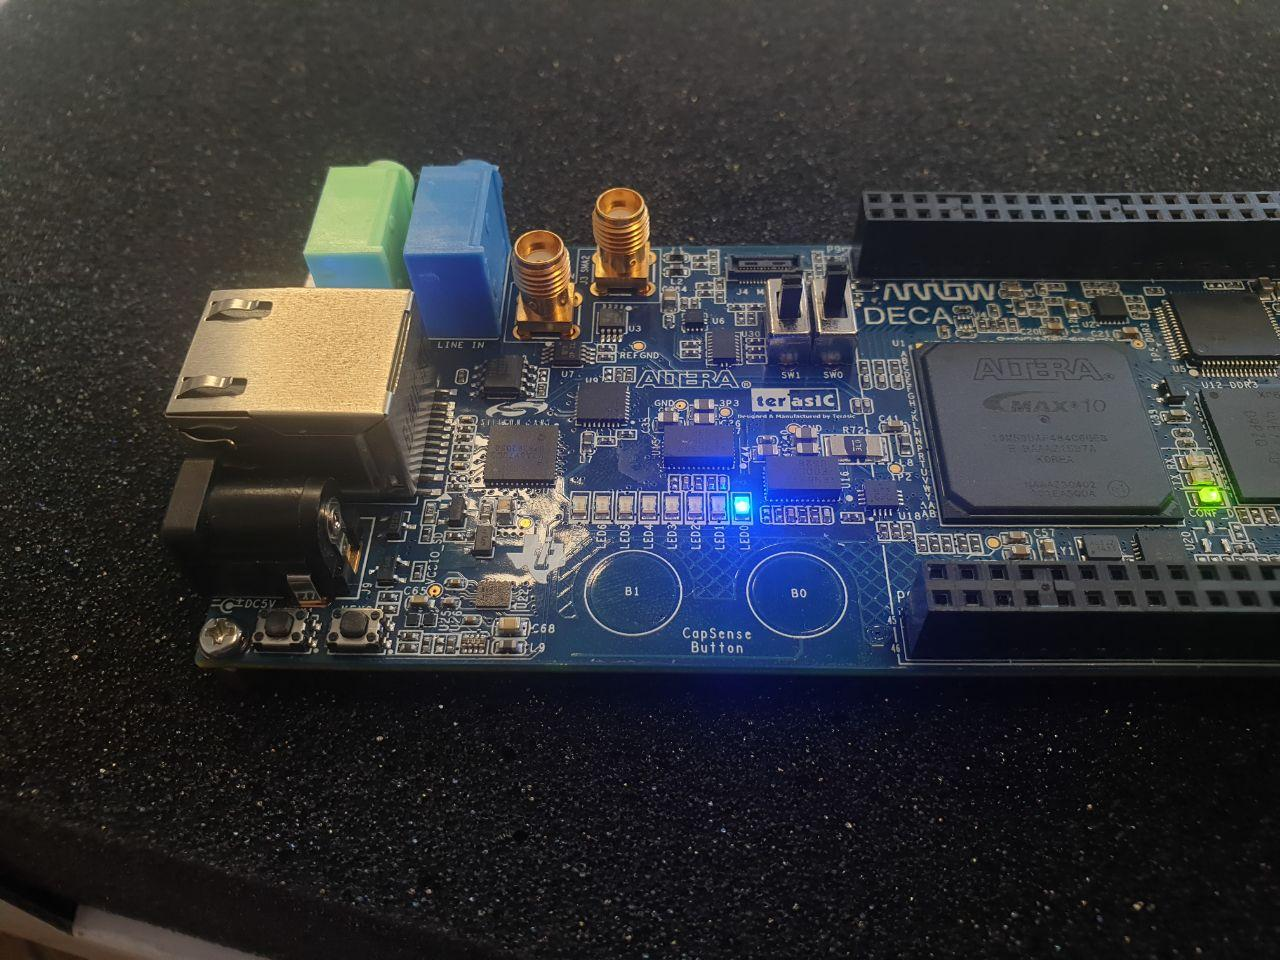
\includegraphics[scale=0.2]{graphics/hardware_output_1} & 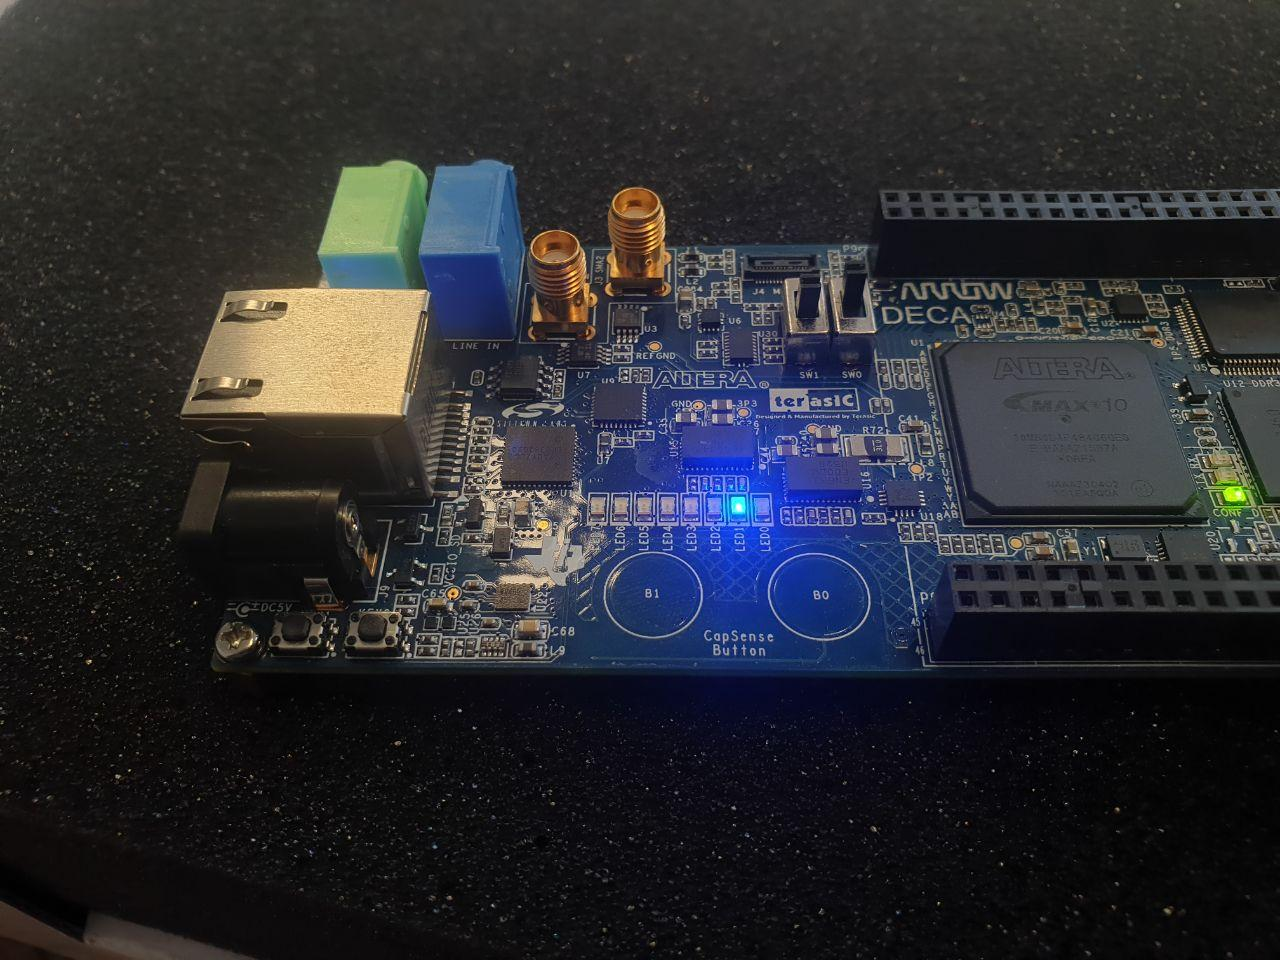
\includegraphics[scale=0.2]{graphics/hardware_output_2} \\
        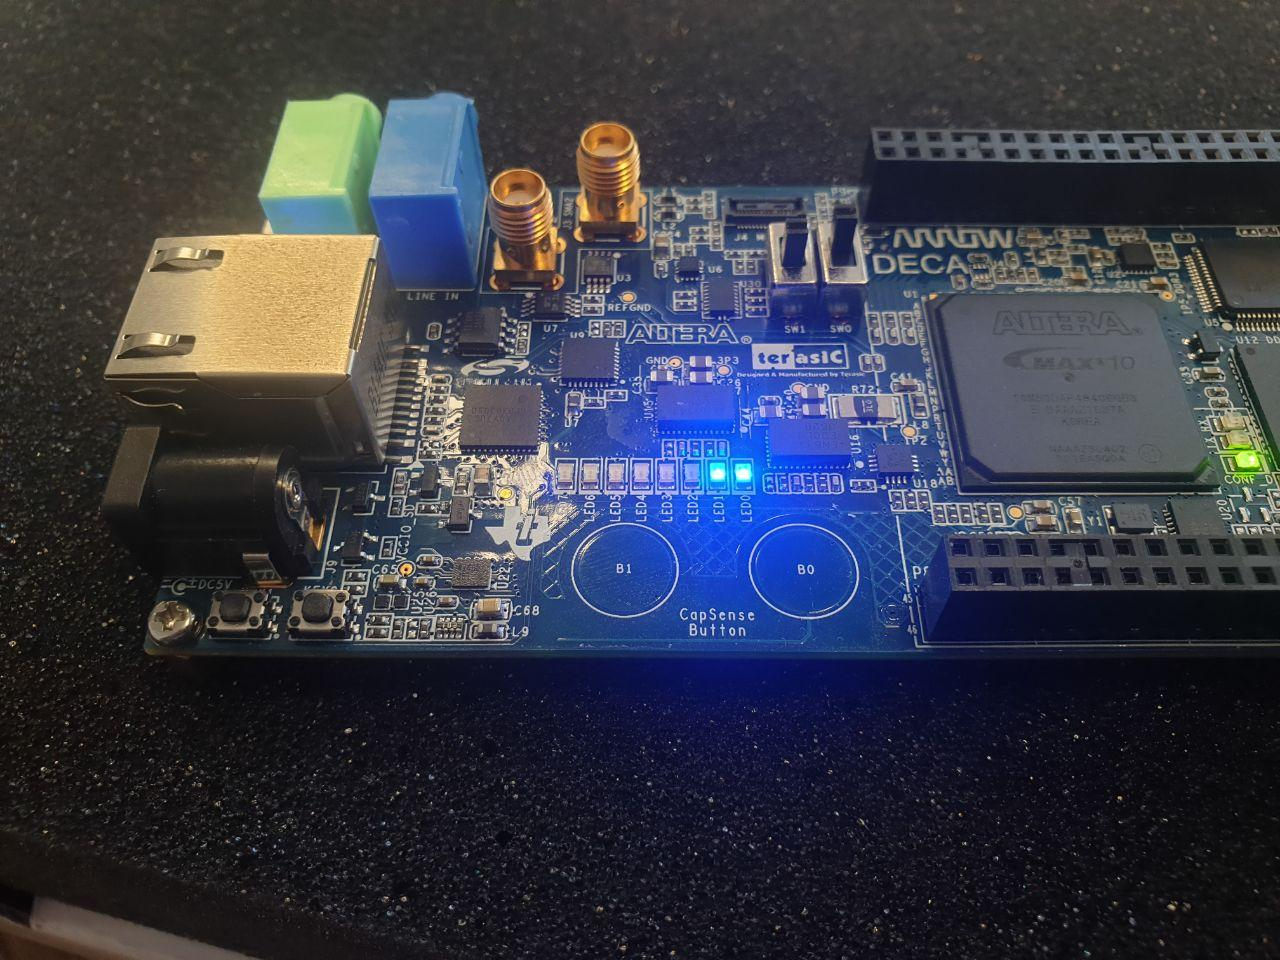
\includegraphics[scale=0.2]{graphics/hardware_output_3} & 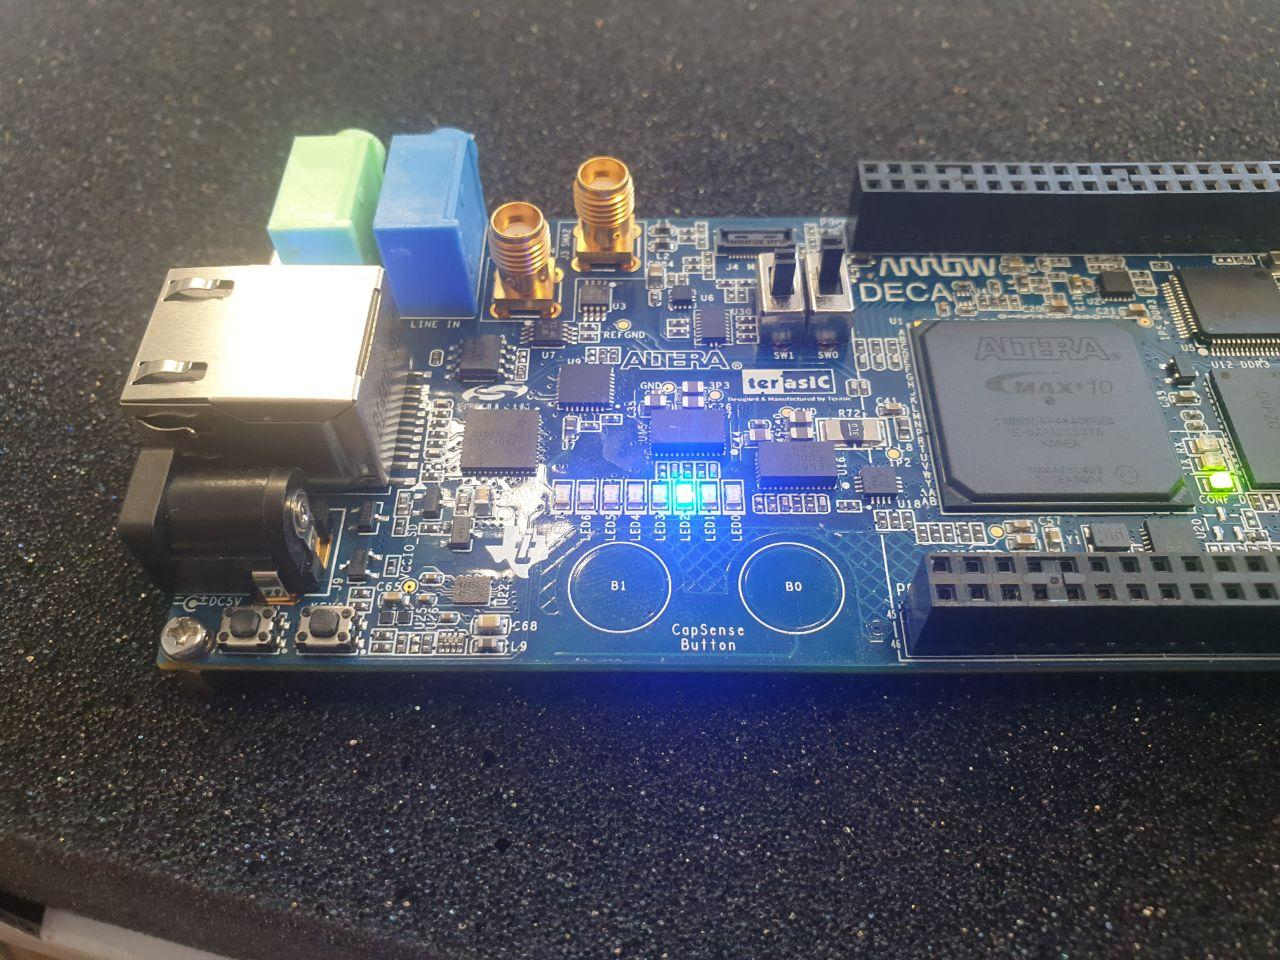
\includegraphics[scale=0.2]{graphics/hardware_output_4} \\
    \end{tabular}
    \caption{Output counting from 1 to 4}
    \label{graphic:output_counting}
\end{table}

\section{Sample Input Program}
This program test the input capabilities of the microcontroller.
It reads the input from the switch and put the value to the output.
The button is configure with pull down configuration, meaning without pressing the button, the input is ground, which is Low.
Upon pressing the button, the input will be 3.3V, which is High.
The output LED is drive accordingly, when input is High, LED is on. When input is Low, LED is off.

\begin{table}[!h]
    \centering
    \caption{Sample Input/Output Program}
    \label{program:sample_io}
    \begin{tabular}{|c|l|l|}
        \hline
        \textbf{Line} & \multicolumn{1}{c|}{\textbf{Instruction}} & \multicolumn{1}{c|}{\textbf{Description}} \\ \hline
        1             & addi x1 x0 16                             & set pin 5 as input                        \\ \hline
        2             & sd x1 x0 1                                &                                           \\ \hline
        3             & L1: ld x3 x0 3                            & read the pin and store into x3            \\ \hline
        4             & and x4 x3 x1                              & Isolate only the input value of pin 5     \\ \hline
        5             & beq x4 x1 L2                              & check if it is 1                          \\ \hline
        6             & addi x5 x0 0                              & set output low if not 1                   \\ \hline
        7             & sd x5 x0 2                                &                                           \\ \hline
        8             & beq x0 x0 L1                              &                                           \\ \hline
        9             & L2: addi x5 x0 1                          & set output high if 1                      \\ \hline
        10            & sd x5 x0 2                                &                                           \\ \hline
        11            & beq x0 x0 L1                              & repeat                                    \\ \hline
    \end{tabular}
\end{table}

As can be observed in Figure \ref{graphic:input_on_off}, the LED is on when the button is pressed and is off when the button is released.\
\begin{table}
    \centering
    \begin{tabular}{cc}
        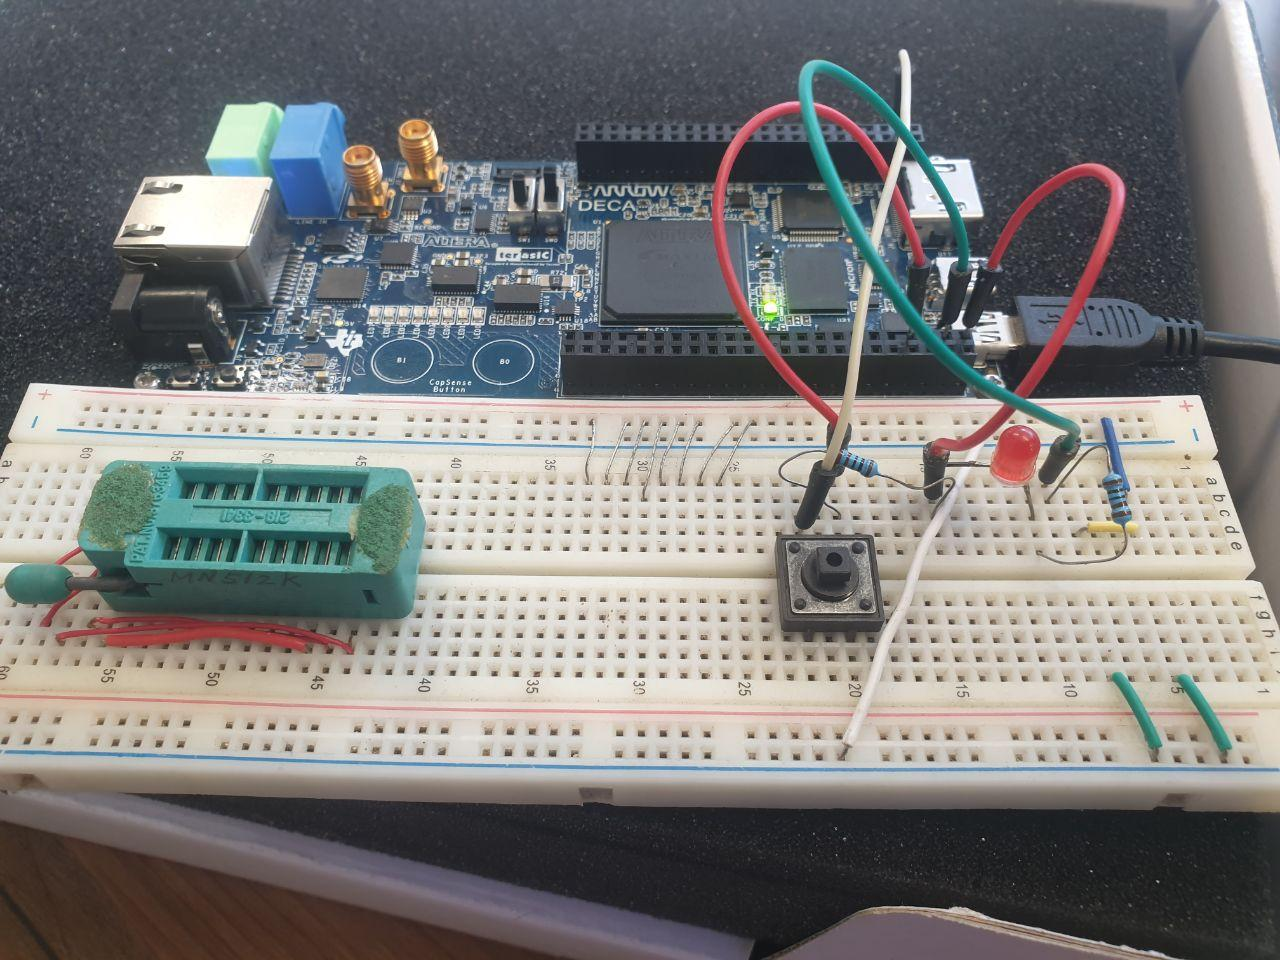
\includegraphics[scale=0.2]{graphics/hardware_input_off} & 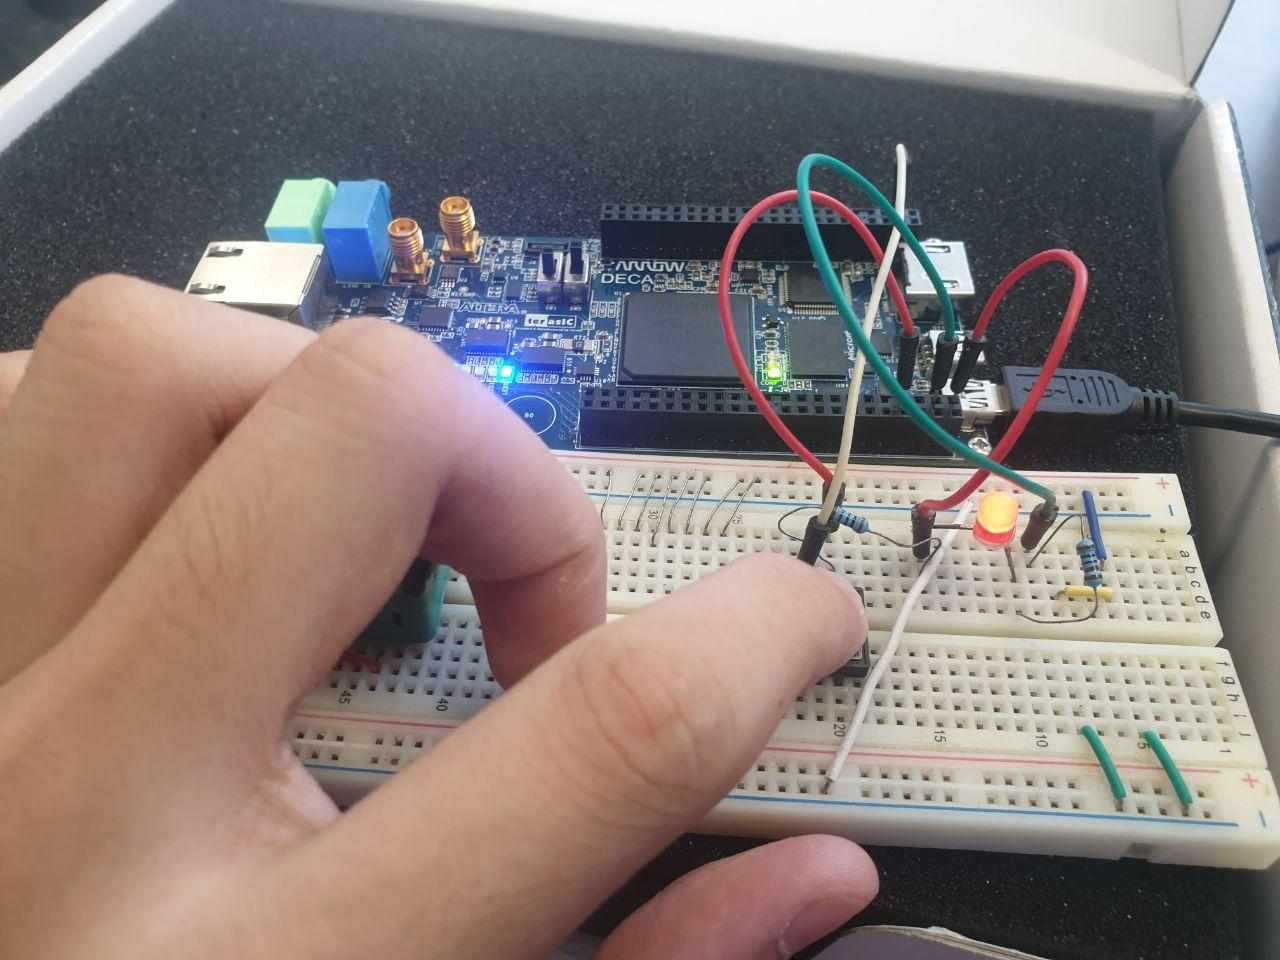
\includegraphics[scale=0.2]{graphics/hardware_input_on}
    \end{tabular}
    \caption{LED turning on button press}
    \label{graphic:input_on_off}
\end{table}

\newpage
\section{Sample UART Transmission Program}
This program tests the transmission of data from UART1 on special I/O.
The program first load the data of 682(1010101010) into the UART1 data write register in Data Memory.
When start signal in UART1 Control register is set, the hardware should start transmitting 4 packet of data, each carrying 1 byte of data.
After that, the TX line should stay in idle state.

\begin{table}[!h]
    \centering
    \caption{Sample UART1 Transmission Program}
    \label{program:sample_uart}
    \begin{tabular}{|c|l|l|}
        \hline
        \textbf{Line} & \multicolumn{1}{c|}{\textbf{Instruction}} & \multicolumn{1}{c|}{\textbf{Description}}    \\ \hline
        1             & addi x1 x0 0                              & clear the control of UART1                   \\ \hline
        2             & sd x1 x0 4                                &                                              \\ \hline
        3             & addi x1 x0 682                            & set the 682 as data to be transmitted        \\ \hline
        4             & sd x1 x0 11                               &                                              \\ \hline
        5             & addi x1 x0 1                              & begin transmitting                           \\ \hline
        6             & sd x1 x0 4                                &                                              \\ \hline
        7             & addi x1 x0 0                              & clear transmitting to only transmit one data \\ \hline
        8             & sd x1 x0 4                                &                                              \\ \hline
        9             & L1:                                       & set output high if 1                         \\ \hline
        10            & beq x0 x0 L1                              & loop                                         \\ \hline
    \end{tabular}
\end{table}

As can be seen in Figure \ref{graphic:hardware_uart}, the data is transmitted and it captured by the oscilloscope.
All four packets of data can be observed as well.

\insertGraphic{hardware_uart}{0.5}{0}{UART1 Transmitting Data}{graphic:hardware_uart}

\chapter{Conclusion}
Building a simple microcontroller using the RISC-V architecture represents an exciting and innovative area of 
research in computer science and embedded systems. 
The RISC-V instruction set architecture (ISA) provides a flexible and open-source foundation for designing 
custom microcontrollers tailored to specific applications. 
Here is a conclusion on this work of building a simple microcontroller using RISC-V:

\paragraph*{Open-Source Advantages}
The use of RISC-V as the basis for a microcontroller offers significant advantages, notably openness and flexibility. Researchers and developers can access and modify the ISA freely, fostering innovation and enabling customized solutions for diverse applications.
\paragraph*{Scalability}
RISC-V microcontrollers can be designed to scale from simple, low-power devices to more complex systems, making them suitable for a wide range of use cases. This scalability allows researchers to explore various design choices and trade-offs.
\paragraph*{Educational Value}
Building a simple RISC-V microcontroller is an educational endeavor with practical benefits. It provides opportunities for students and enthusiasts to learn about computer architecture, digital design, and embedded systems by working with a real-world, open-source ISA.
\paragraph*{Customization}
Researchers can tailor the microcontroller's architecture and features to meet specific application requirements. This customization can lead to energy-efficient, cost-effective solutions optimized for particular tasks.
\paragraph*{Challenges and Trade-Offs}
While RISC-V offers flexibility, designing a microcontroller from scratch can be complex and time-consuming. Researchers must carefully consider trade-offs between power efficiency, performance, and resource utilization to achieve their design goals.

Over the course of this work, it can also be concluded that the designed microcontroller works both in simulation and with hardware and can be expanded at will.
There are many potential optimazations that can be done such as choosing a better architecture and building a more coincise hardware. 

\section{Further Works}
In order to fully usable as a microcontroller, there are many features that will need to be implemented. Below is a list of some potential features
\begin{itemize}
    \item More Instructions
    \item Interrupts
    \item Timers
    \item Support for procedures
    \item Multiplexing special and general I/O
\end{itemize}


\newpage

\begin{appendices}

	\chapter{Some Appendix}

	\section{Source Code}
	\label{appendix:source}
	Source Codes can be found on the GitHub Page: \url{https://github.com/kaung-minkhant/risc-v-deca}

	\section{Requirements}
	\subsection{Hardware and Software Requirements}
	Hardware and software requirements are as follow
	\begin{enumerate}
		\item Arrow Deca FPGA Development Board
		\item Intel Quartus Prime Lite Software
		\item ModelSim Lite simultation Software
	\end{enumerate}
	\subsection{Skill Requirements}
	The following skills are required.
	\begin{enumerate}
		\item VHDL Programming
		\item Computer Organization and Designe for RISC-V ISA
		\item Micro-controller Peripheral Design
		\item Micro-controller Communication Design
		\item Assembly for RISC-V ISA
	\end{enumerate}

	\newpage

	\section{Timeline}
	\insertGraphic{timeline}{0.08}{90}{Timeline of the project}{graphic:timeline}


\end{appendices}

\afterpage{\blankpage}

\addcontentsline{toc}{section}{References}
\bibliography{references}
\bibliographystyle{apalike}

\end{document}
